\documentclass[a4paper,french]{article}

\usepackage{natbib}
\usepackage{graphicx}
\usepackage[french]{babel}
\usepackage[utf8]{inputenc}
\usepackage[T1]{fontenc} 
\usepackage{xcolor}
\usepackage[left=2cm,right=2cm,top=2cm,bottom=2cm]{geometry}
\usepackage{fancyhdr}
\usepackage{lastpage}
\usepackage{import}
\usepackage{enumitem}
\usepackage{todonotes}
\usepackage{hyperref}
\usepackage{float}
\usepackage{subcaption}
\usepackage{caption}
\usepackage{listings}
\usepackage{pdfpages}

%C'est pour afficher les .json proprement

\colorlet{punct}{red!60!black}
\definecolor{background}{HTML}{EEEEEE}
\definecolor{delim}{RGB}{20,105,176}
\colorlet{numb}{magenta!60!black}

\lstdefinelanguage{json}{
    basicstyle=\normalfont\ttfamily,
    numbers=left,
    numberstyle=\scriptsize,
    stepnumber=1,
    numbersep=8pt,
    showstringspaces=false,
    breaklines=true,
    frame=lines,
    backgroundcolor=\color{background},
    literate=
     *{0}{{{\color{numb}0}}}{1}
      {1}{{{\color{numb}1}}}{1}
      {2}{{{\color{numb}2}}}{1}
      {3}{{{\color{numb}3}}}{1}
      {4}{{{\color{numb}4}}}{1}
      {5}{{{\color{numb}5}}}{1}
      {6}{{{\color{numb}6}}}{1}
      {7}{{{\color{numb}7}}}{1}
      {8}{{{\color{numb}8}}}{1}
      {9}{{{\color{numb}9}}}{1}
      {:}{{{\color{punct}{:}}}}{1}
      {,}{{{\color{punct}{,}}}}{1}
      {\{}{{{\color{delim}{\{}}}}{1}
      {\}}{{{\color{delim}{\}}}}}{1}
      {[}{{{\color{delim}{[}}}}{1}
      {]}{{{\color{delim}{]}}}}{1},
}

\usepackage{color}
\definecolor{freeblue}{rgb}{0.25,0.41,0.88}

\title{Informations de PFA}
\author{PFA}
\date{\date}

\pagestyle{fancy}

\renewcommand{\headrulewidth}{1pt}
\fancyhead[L]{\textsc{Rapport}}
\fancyhead[C]{}
\fancyhead[R]{\leftmark}

\renewcommand{\footrulewidth}{1pt}
\fancyfoot[L]{PFA 12}
\fancyfoot[C]{}
\fancyfoot[R]{\textbf{\thepage/\pageref{RealLastPage}}}

\begin{document}
\begin{titlepage}
\centering
\vspace*{1\baselineskip}
\LARGE{\textsc{Filière Informatique - Semestre 8}} \\
\vspace*{\baselineskip}
\LARGE{\textsc{\bfseries{Rapport}}} \\

\vspace*{2\baselineskip}
\hrulefill \\[0.4cm]
{ \Huge \bfseries Application d'assistant vocal sur \\[0.4cm] }
{ \Huge \bfseries Reachy Mini \\[0.4cm] }
\hrulefill \\[1.5cm]
\vspace*{\baselineskip}
\centering
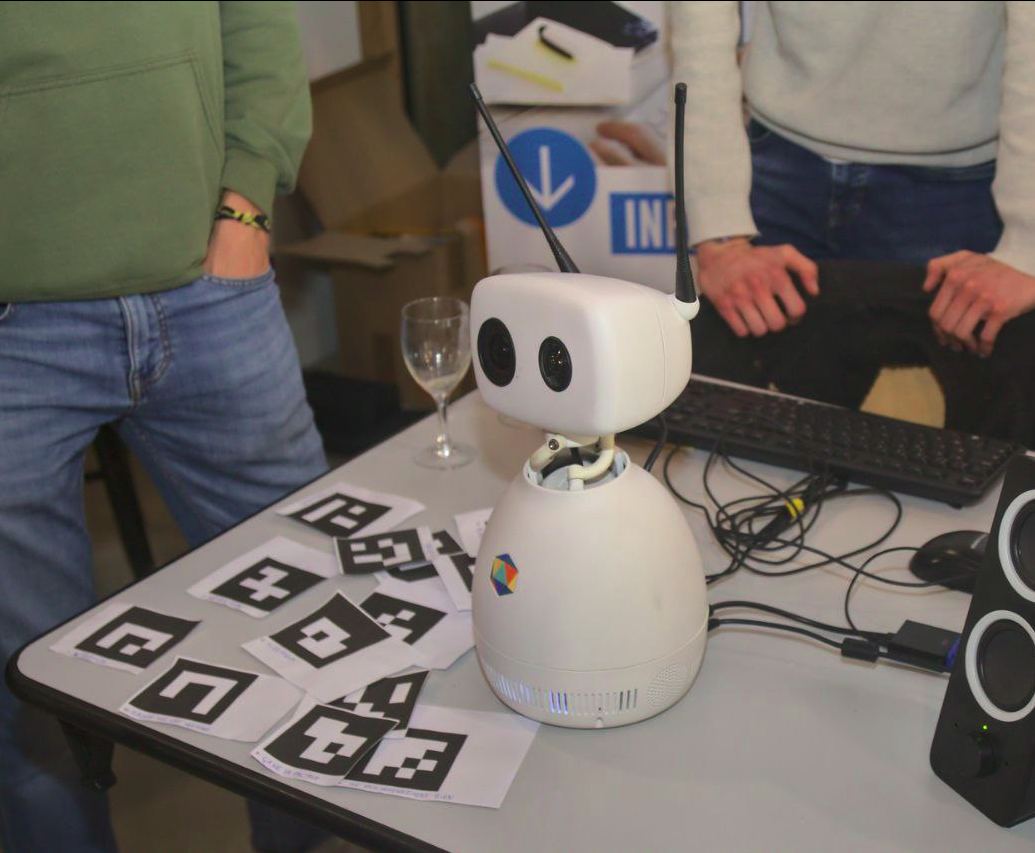
\includegraphics[scale=0.25]{figures/reachy_sp.png}
\\
\vspace*{2\baselineskip}

\begin{minipage}[b]{0.40\linewidth}
        \flushleft 
        \large
        \emph{Auteurs :} \\
        \textsc{Boudeau} Benjamin\\
        \textsc{Dieudonné} Clara \\
        \textsc{Elfani} Hamza \\
        \textsc{Lamhamdi} Aymane \\
        \textsc{Marais} Lucas \\
        \textsc{Raïs} Sylvain \\
        \textsc{Zizouan} Widad\\
    \end{minipage} \hfill
    \begin{minipage}[b]{0.40\linewidth}
        \flushright 
        \large 
        \emph{Encadrant :} \\
        \textsc{Rollet} Antoine \\
        \textsc{Morandat} Floréal \\
        \emph{Client :} \\
        \textsc{N'guyen} Steve \\
    \end{minipage} \hfill

\end{titlepage}

\tableofcontents
\newpage

\section{Introduction}
%Présentation de l'API
Le Projet au Fil de l'Année, aussi appelé PFA, consiste en la réalisation d'un projet concret proposé par un client à 7 élèves ingénieurs de l'ENSEIRB-MATMECA. Ce rapport a pour but de détailler la réalisation du projet concernant le robot Reachy Mini de l'entreprise Pollen Robotics. Ce projet a été proposé par \textsc{N'guyen} Steve, client membre de l'entreprise ayant développé le robot. \\

\textbf{Reachy Mini} \\ \\
Le robot Reachy Mini est un robot articulé. Cependant il se distingue des robots habituels et notamment de son grand frère, le robot Reachy, par son unique buste dépourvu de jambes. Ce sont sa tête, et ses antennes qui sont articulées à 360°, dans la limite des câbles électriques passant par le coup et permettant l'alimentation de la caméra située dans la tête. En effet, le robot possède deux caméras à la place de ses yeux, il peut donc voir et capter l'environnement autour de lui. Monté sur un PC au processeur Intel NUC et un Google Coral, embarquant un micro multi-directionnel et deux haut-parleurs, le robot possède les outils nécessaires à l'analyse de l'environnement et l'interaction avec le monde qui l'entoure. \\

\textbf{Pollen Robotics} \\ \\
Fondée en 2016 par d'anciens chercheurs, Pollen Robotics est une entreprise qui rassemble des personnes talentueuses et indépendantes dans le but de fournir des produits et des applications accessibles et open source. L'entreprise participe donc à l'évolution de l'IA et de la robotique et est motrice à son intégration dans la vie quotidienne. Elle expose ainsi son robot principal Reachy sur de nombreux évènements autour de l'informatique, la robotique et l'intelligence artificielle. \\


\begin{figure}[H]
    \centering
    
\includegraphics[scale = 0.25]{figures/pollen_robotics.jpg}
    \caption{Logo de Pollen Robotics}
    \label{fig:logo}
\end{figure}

\textbf{Le projet} \\ \\
Le travail demandé par le client pour réaliser ce projet était de programmer Reachy afin qu'il se rapproche d'un assistant vocal du type Amazon Echo, ou Google Home. La reconnaissance vocale, le traitement d'images, la synthèse vocale et les mouvements du robot étaient donc à implémenter. \\

L'objectif principal du projet était la présentation du robot lors des 100 ans de l'ENSEIRB-MATMECA, le 8 avril 2022. Cependant, l'événement a été déplacé au 30 septembre. L'objectif principal a donc été la présentation du robot lors de la soirée des partenaires de l'école, événement qui sera détaillé dans ce rapport. Le robot devait alors être capable de prendre des photos, et interagir avec les utilisateurs. \\
D'autres fonctionnalités demandées par le client consistaient à pouvoir demander les conditions de surf en un lieu et une journée précise. Le robot devait ainsi aller sur internet et effectuer cette recherche avant d'informer l'utilisateur avec la réponse. \\

Ce rapport se décompose en plusieurs parties, la première présentera l'organisation du projet tout en respectant les méthodes agiles. Ensuite, nous présenterons l'architecture de l'implémentation de notre projet avant de présenter les différentes attentes du projet et de les comparer à la réalisation effectuée. Enfin, nous présenterons le manuel d'utilisation du robot et ses limites avant de finir par présenter l'événement de la soirée partenaires.

\newpage

\section{Organisation et méthodes agiles}
Afin d'organiser la réalisation du projet, il a été nécessaire de respecter les méthodes agiles. Ce projet a ainsi été organisé autour de sprints permettant le développement de solutions et la consultation avec le client pour vérifier le bon respect des contraintes et besoins. \\

Afin de coordonner le travail entre les 7 membres du groupe, un gestionnaire de tâches a été utilisé. Pour réaliser ce projet, c'est ClickUp qui a été choisi comme gestionnaire.

\subsection{Utilisation de ClickUp}
ClickUp permet de centraliser les fonctions collaboratives d'un projet. L'outil regroupe en effet de nombreuses fonctionnalités et permet ainsi de n'utiliser qu'une unique interface de gestion au lieu de multiplier les outils. ClickUp facilite donc la coordination au sein du groupe. L'outil permet de créer des listes de tâches simples et des listes plus complexes avec des sous-tâches, attribution de rôle, ... Il permet également la génération de calendriers correspondant à ces tâches et leurs dates de réalisation ou deadline. Les différents diagrammes de Gantt peuvent ainsi être générés directement sur ClickUp en liant les tâches entre elles avec des dépendances. \\

Certains outils comme le tableau blanc, ou les notes sont aussi utiles pour la coordination du groupe, notamment avec les réunions à distances qui sont facilitées par cet outil. \\

Ainsi, nous avons choisi d'utiliser ClickUp pour son interface intuitive, sa modernité et ses nombreuses fonctionnalités permettant de centraliser une grande partie de la gestion du projet sur un seul outil.

\begin{figure}[H]
    \centering
    
\includegraphics[scale=0.2]{figures/clickup-logo.png}
    \caption{Logo ClickUp}
\end{figure}

\subsection{Répartition des tâches}
En fonction des besoins fonctionnels et non fonctionnels identifiés entre l'équipe et le client au début du projet, différentes équipes ont été formées pour pouvoir avancer le projet en parallèle. Puis chaque implémentation interdépendantes ont été regroupées pour permettre le fonctionnement global du robot. \\

L'un des premiers besoins fonctionnels était les mouvements du robot. En effet, lors de son interaction avec les utilisateurs, ce dernier devait être possible de réaliser des mouvements afin de notamment regarder l'interlocuteur, mais aussi faire des émotions telles qu'être content, ou triste. \\

Ainsi, Lucas et Clara ont formé la première sous-équipe et se sont concentrés sur les parties liées au mouvement du robot. L'utilisation de l'API \texttt{reachy-sdk} a permis d'utiliser les fonctions bas niveau de Reachy pour implémenter tous les mouvements réalisables par le robot. \\

Ensuite, le robot devait être en mesure de parler afin d'interagir avec un potentiel utilisateur. Aymane et Hamza ont donc étudié la synthèse vocale en cherchant à donner au robot une voix cohérente et en créant un système de parole. \\

Pour pouvoir parler aux utilisateurs, il était nécessaire que le robot comprenne ce qu'ils pouvaient lui dire. La reconnaissance vocale a donc constitué une troisième partie du projet. Benjamin et Widad ont ainsi travaillé sur la compréhension d'un texte oral et son analyse par le robot. Ensuite Benjamin s'est tourné vers la mise en place de machines à états plus complexes et Widad sur la mise en place des conversations avancées. \\

Enfin, comme l'un des objectifs était la prise de photo par le robot, Sylvain a constitué la dernière sous-équipe en travaillant avec l'API \texttt{OpenCV} pour analyser l'image captée par les caméras du robot et implémenter la prise de photos. \\

Quatre équipes distinctes ont ainsi été constituées. Certains sous-objectifs du projet tels que la mise en place de la machine à états permettant le fonctionnement du robot ou encore la mise en place des actions parallèles, ont entraîné la création de nouvelles sous-équipes avec des tâches en parallèle de leurs tâches principales. \\

ClickUp a permis de centraliser les étapes de la réalisation de ces différentes tâches. Le maintien régulier de l'avancée de ces tâches permettait donc de connaître le retard pris sur certaines étapes ou l'avancée prise sur d'autres, et donc de corriger en apportant plus d'aide sur une étape plutôt que sur une autre. \\ Ainsi, le diagramme de Gantt initial a évolué au cours du projet. En effet, ces retards ou avancées ont eu des impacts légers sur la planification du projet. \'Egalement, certaines fonctionnalités n'avaient pas été réfléchies de la même façon qu'elles ont été finalement implémentées. Ces légers changements ont donc eu un impact important dans la planification finale du projet, remettant en cause certaines parties du projet ou leur implémentation. \\

\begin{figure}[H]
    \centering
    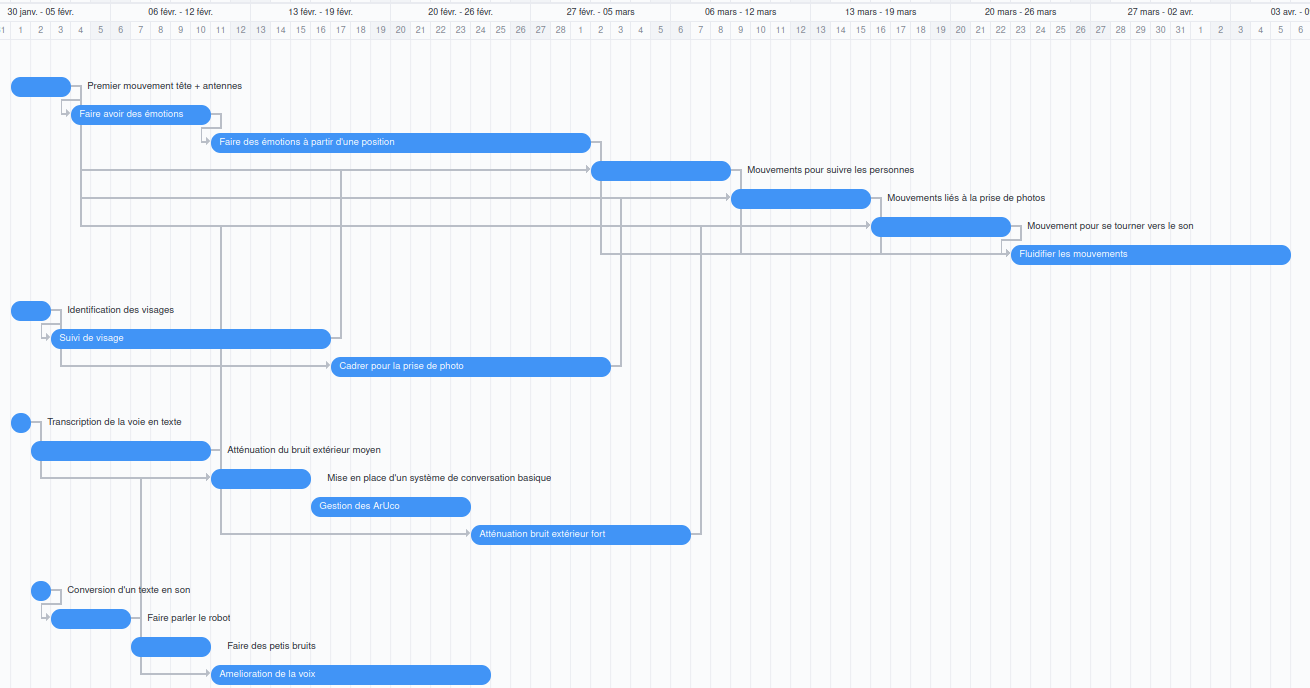
\includegraphics[scale=0.35]{figures/gantt_avant_100_ans.png}
    \caption{GANTT initial avant les 100 ans}
\end{figure}

\begin{figure}[H]
    \centering
    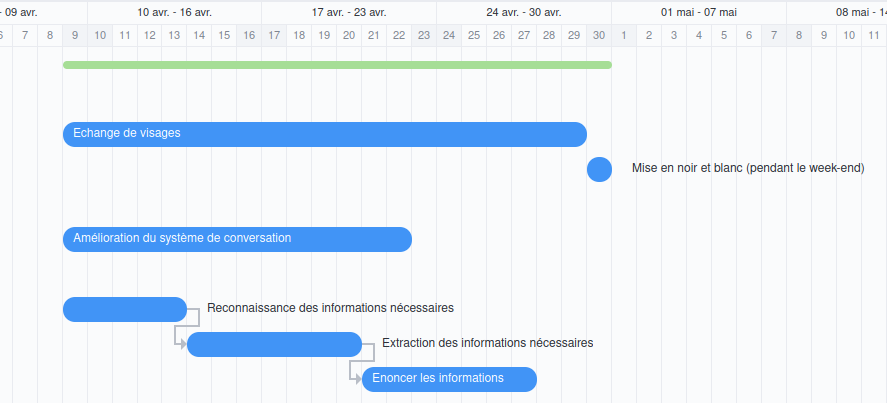
\includegraphics[scale=0.5]{figures/gantt_apres_100_ans.png}
    \caption{GANTT initial après les 100 ans}
\end{figure}

\begin{figure}[H]
    \centering
    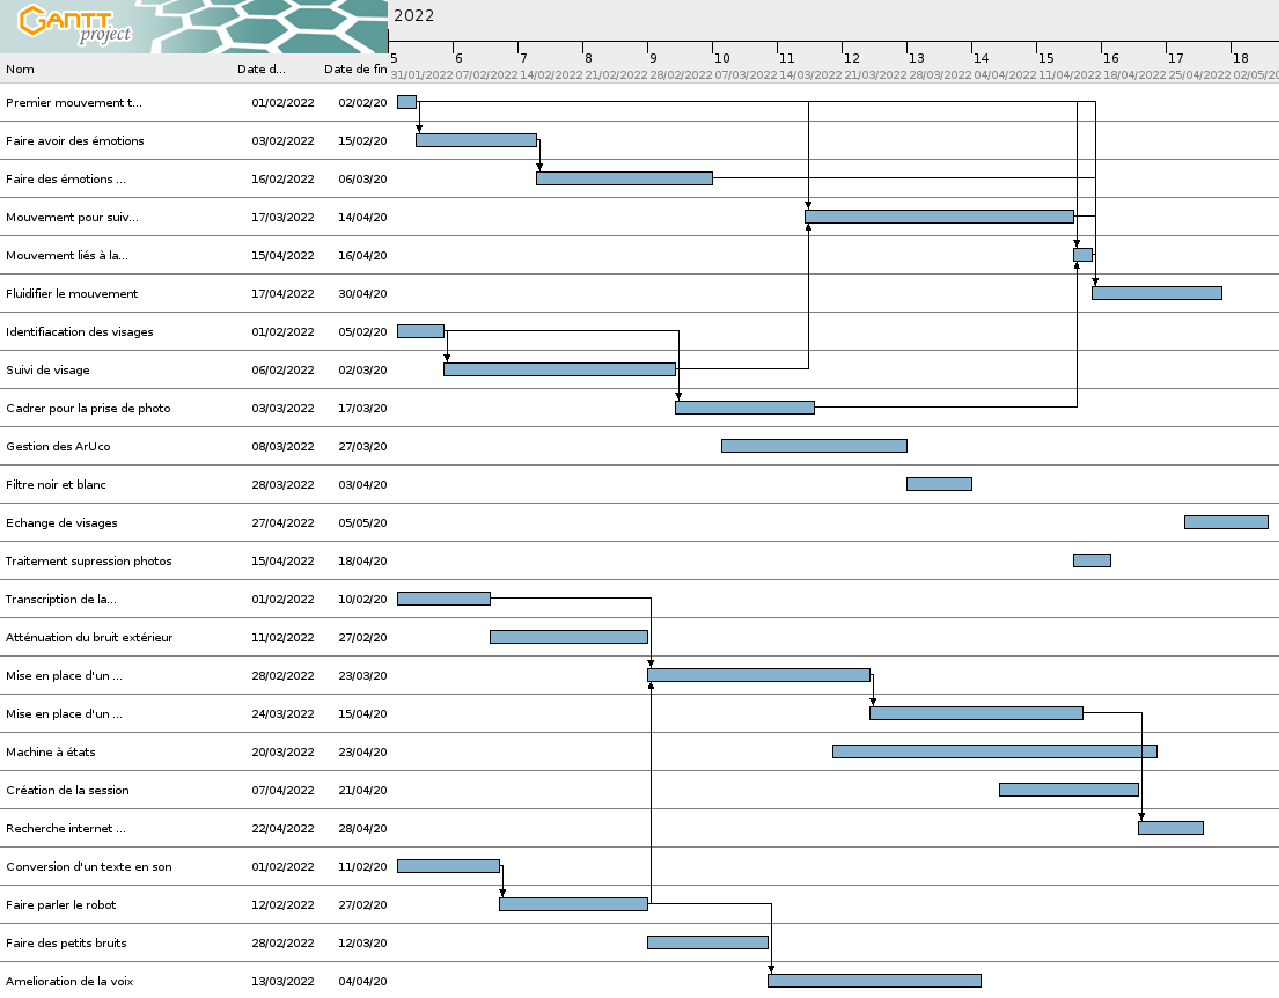
\includegraphics[scale=0.38]{figures/gantt_fin_PFA.png}
    \caption{GANTT final}
\end{figure}

\subsection{Utilisation de Github}
Pour permettre le partage du code au sein de l'équipe mais également avec l'encadrant, plusieurs solutions étaient possibles. \\

La première consistait à utiliser les serveurs de l'école et héberger le projet sur un dépôt git lié à la forge de l'école. Cependant, suite à quelques latences fréquentes ayant eu lieu en début d'années sur Thor, nous avons choisi de ne pas utiliser cette méthode. \\

Ensuite, nous avions le choix entre plusieurs gestionnaires de dépôt git tels que Github ou Gitlab. C'est avec unanimité que nous avons choisi Github, étant tous déjà utilisateurs de cet outil et familiers avec son utilisation. \\

Le robot a d'ailleurs été connecté au compte Github de Lucas. De nombreux commits ayant été réalisés depuis le robot, ce compte possède une grande partie du code du projet, bien que toute l'équipe ait travaillé et codé avec le robot.

\subsection{Organisation des sprints et livrables}
Le management du projet a été organisé selon les principes des méthodes agiles. Pour cela, différents sprints ont été réalisés. Un sprint consistait en la mise en commun d'objectifs avec l'encadrant et/ou le client, puis la réalisation de ces objectifs pendant 2 semaines avant une deuxième réunion de validation de la réalisation. \\
Différents livrables ont ainsi pu être présentés respectant les étapes de validation de ces sprints. \\

Le rythme moyen de réunions consistait à réaliser une réunion par semaine soit avec l'encadrant, soit avec le client. Cependant, nous avons eu un deuxième encadrant (Mr \textsc{Morandat}) au milieu du projet, ce qui a légèrement impacté ce rythme régulier de réunion. En effet, ce nouveau regard extérieur sur le projet, a permis de lever de nouvelles idées notamment sur la gestion des mouvements du robot et de la machine à états. Il a donc fallu revoir certaines notions de l'implémentation et donc mettre en stand-by la réalisation du livrable suivant pour le client. \\

Nous avons, par ces changements, permettant une implémentation plus rapide, pu reprendre le rythme normal des sprints par la suite. \\

Afin de développer les livrables, nous avons utilisé différentes branches du dépôt git, pouvant ainsi conserver un livrable fonctionnel et continuer de développer la suite du projet en parallèle. De plus, ces branches ont permis de tester différentes solutions à différents problèmes sans impacter la globalité du projet. \\ La bonne intégrité de la branche principale (\texttt{master}), est en effet un des aspects caractéristiques des méthodes agiles. Au maximum, les commit et pushs étaient donc réalisés sur une branche parallèle puis intégrée au reste du code après validation.

\subsection{Les tests réalisés}
Afin de réaliser des tests sur l'implémentation du projet, nous avons utilisé différentes méthodes. \\

La première consistait en tests de recette. En effet, la plupart des fonctions du robot étant des fonctions de mouvement utilisant l'API, elles ne retournent pas forcément de valeurs. Il a donc été visuellement possible de tester certaines parties du code en appelant certaines fonctions et en observant leur bonne exécution. \\

Par exemple, tout le code lié aux photos ne retourne pas de valeurs mais manipule des fonctions. Pour les tester, nous avons donc vérifié la bonne réalisation des attentes par le robot. \\

Nous avons cependant réalisé quelques tests unitaires sur certaines fonctions comme \texttt{inverse\_kinematic} par exemple en vérifiant sa valeur de retour qui parfois est \textit{null} car elle n'a pas trouvé de solution au quaternion. \\

En ce qui concerne la synthèse vocale ou la reconnaissance vocale, il n'était possible de réaliser que des tests visuels, tests de recette. En effet, il n'est pas possible de tester si le robot capte bien le son autrement qu'en parlant et regardant ce qu'il détecte. Pareil pour la synthèse ou il est impossible de tester autrement qu'en faisant parler le robot et vérifiant qu'il a dit la bonne chose. \\

Ainsi, ce projet se portait peu à l'utilisation de test unitaire ou d'intégrité. Cependant les tests de recettes ont été très utilisés.

\section{Architecture de notre projet}
Un aspect important du projet est aussi l'organisation et l'architecture de notre code afin de le rendre plus fonctionnel et modulable.
\subsection{Organisation de notre code}
L'implémentation de l'ensemble du code du projet constituant un nombre important de lignes de code, nous avons donc séparé le code du projet en plusieurs fichiers sources. Chaque fichier correspondant à une partie du projet (Mouvement, Traitement d'image, ...). En plus des fichiers qui codent l'implémentation du projet, il y a aussi des fichiers permettant la description et l'exécution du projet. \\
Nous avons donc créé différents dossiers pour organiser tout cela. Dans un premier temps, nous avons fait une séparation entre les fichiers qui sont utilisés par le code : \texttt{assets}, le code en lui-même : \texttt{src}, les fichiers créés par le code : \texttt{tmp} et les tests : \texttt{tst}.\\

Le dossier \texttt{assets} contient l'ensemble des commandes vocales pour passer d'un état à un autre, les fichiers \texttt{json}, pour créer la machine à états dont le fonctionnement sera détaillé dans la partie \ref{section_machine_etat}, les sons que Reachy émet.\\

Le dossier \texttt{src} est séparé en 6 parties, un dossier contenant le code pour la détection d'image \textit{détection}, un pour la session, détaillé en \ref{section_session}, un pour la synthèse vocale \textit{speech}, un pour les machines à états \textit{state\_machine}, et un pour la gestion mémoires pour l'enregistrement des photos \textit{storage\_management}. Enfin, certains fichiers ne faisant pas partie d'un groupe de fichiers, sont simplement dans le répertoire \texttt{src} comme le mouvement ou la reconnaissance vocale.\\

Le dossier \texttt{tmp} permet de stocker les images et les sons enregistrés par le robot.\\

Le dossier \texttt{tst} contient les fichiers permettant de vérifier le fonctionnement de notre code.\\

\begin{figure}[H]
    \centering
    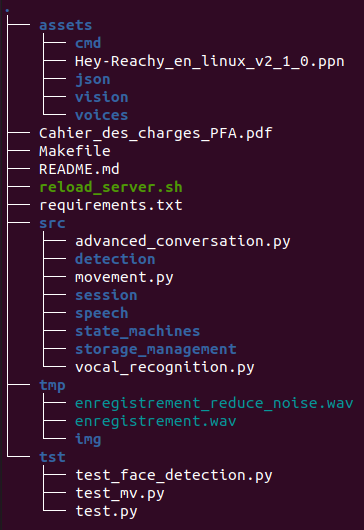
\includegraphics[scale = 0.5]{figures/tree_pfa.png}
    \caption{Arborescence de notre code}
    \label{fig:tree}
\end{figure}

\subsection{Utilisation d'une session} \label{section_session}
Pour permettre l'abstraction des fonctions bas niveau de l'api \textbf{reachy-sdk}, nous avons utilisé le principe de session.
\subsubsection{Première implémentation}
Afin de gérer les mouvements du robot, nous avions initialement créé un simple fichier \texttt{movement.py} qui contenait les fonctions des mouvements telles que celles des émotions (\texttt{sad, happy, listen, ...}), celles permettant le mouvement du robot pour suivre un visage, et celles permettant le mouvement des antennes. \\

Ce fichier constituait ainsi une classe \texttt{Movement} qui avait alors un \texttt{ReachySDK} comme attribut, et la connexion au robot était réalisée par l'intermédiaire de cet attribut. Cependant, l'usage de la caméra nécessitait également une connexion au robot. Il fallait donc se connecter au robot de deux façons différentes dans le main de la machine à états afin de créer ces liens.

\subsubsection{Soucis engendrés}
Avec cette implémentation, l'utilisation du robot nécessitait alors la connexion à ce dernier de deux façons. Nous avions donc des problèmes de liens avec le robot. En effet, la plupart du temps, il y avait deux instances de créées et non une unique qui servait pour le mouvement et la caméra. \\

\'Egalement, avec cette méthode, la connexion au robot étant réalisée dans le main, il y avait du code gérant la connexion dans la machine à états, alors qu'il n'y a pas de liens directs entre les deux modules.
Ainsi, il fallait trouver un moyen de ne réaliser qu'une unique connexion et hors du fichier de la machine à états. \\

De plus, afin de réaliser les tests, nous avions besoin d'un faussaire, c'est-à-dire un faux robot, permettant de tester nos fonctions sans nécessité de connexion au réel robot. Avec cette implémentation, il était donc nécessaire de créer deux fichiers \texttt{movement.py} et \texttt{mock\_movement.py}. Or cela impliquait de la duplication de code.

\subsubsection{Solution envisagée}
La solution envisagée a consisté en la création d'une session. Une session est un objet manipulé par les états et transitions de la machine à états et permettant la connexion au robot depuis la création du contexte de cette machine à états. \\

La session est donc une classe abstraite des fonctions bas niveau du robot utilisée dans l'intégralité du projet (mouvement, caméra, ...). Ensuite, nous avons pu développer deux sous-classes qui étendent cette classe abstraite : \texttt{ReachySession} et \texttt{FakeSession}. Ainsi, la classe correspondant à la session d'un réel robot étend les fonctions bas niveau en appelant celles du robot alors que la session faussaire, ne réalise que des affichages permettant de voir quelles fonctions ont été appelées. \\

Le fichier permettant les mouvements implémente ainsi les fonctions des mouvements en passant en paramètre une session. Ainsi, chaque mouvement est réalisé sur une session, et c'est en fonction de la session passée en paramètre que ces mouvements sont réalisés sur le robot ou sur le faussaire. \\ Les mouvements ne sont donc plus une classe mais un simple fichier de définition des méthodes permettant au robot de bouger. \\

Ainsi, depuis la machine à états, on peut appeler les fonctions de mouvement avec comme paramètre le champ \textit{session} du contexte de la machine à états.

\subsection{Utilisation d'une machine à états}
\label{section_machine_etat}
Dès le début du PFA nous avons choisi d'utiliser une machine à états afin de spécifier les fonctionnalités du robot dans le cahier des charges. Nous avons choisi cette manière de spécifier car celle-ci se prête bien pour un robot, le Reachy peut s'apparenter à un ensemble d'états et de transitions avec des prédicats qui permettent de cheminer correctement dans cet ensemble d'états. Lorsque nous avons commencé à coder, l'une des premières choses que nous avons faite a été d'implémenter cette machine à états. Cela s'est fait en plusieurs temps que nous allons expliquer maintenant.

\subsubsection{Première implémentation}

La première implémentation de la machine à états se basait sur un système de dictionnaires. Il y avait un dictionnaire avec comme clé les noms des états et comme valeur la fonction associée à l'état. Chaque fonction d'état commençait par effectuer l'action de l'état puis ensuite il y avait une phase de détection de transition implémentée par une succession d'instructions conditionnelles. \\ 

Cette méthode a vite montré ses limites, lorsqu'il s'agissait de rajouter une transition, la fonction de l'état associé devenait rapidement illisible. De plus, il était compliqué de créer d'autres machines à états sans devoir tout refaire. C'est pourquoi, avec les conseils de M. Morandat, nous nous sommes lancés dans l'implémentation d'un objet State\_Machine dont le but était de généraliser cette notion de machine à états et de pouvoir ainsi créer des sous machines de tests qui font par exemple exclusivement la photo ou bien la conversation. 

\subsubsection{Implémentation de la machine à états généralisée} \label{subsubsec:StMaGeneral}

Afin de généraliser la notion de machine à états il a fallu se poser la question des éléments qui la composent. Il y a donc les états et les transitions, ces éléments sont eux-mêmes découpés en sous-éléments. Pour un état nous trouvons son action et son ensemble de transitions sortantes. Pour une transition il y a un état de sortie, un prédicat ainsi qu'une action. Lors des débuts de la généralisation de l'objet State\_Machine, nous avons créé un objet pour les états et un autre pour les transitions. Finalement nous avons trouvé cela plus simple de rester sur seulement un objet State\_Machine et de représenter les états et les transitions de manières différentes. \\

Afin d'expliquer tout cela plus simplement, nous allons nous baser sur la Figure \ref{fig:statemachine} qui résume la structure de la State\_Machine. 

\begin{figure}[H]
    \centering
    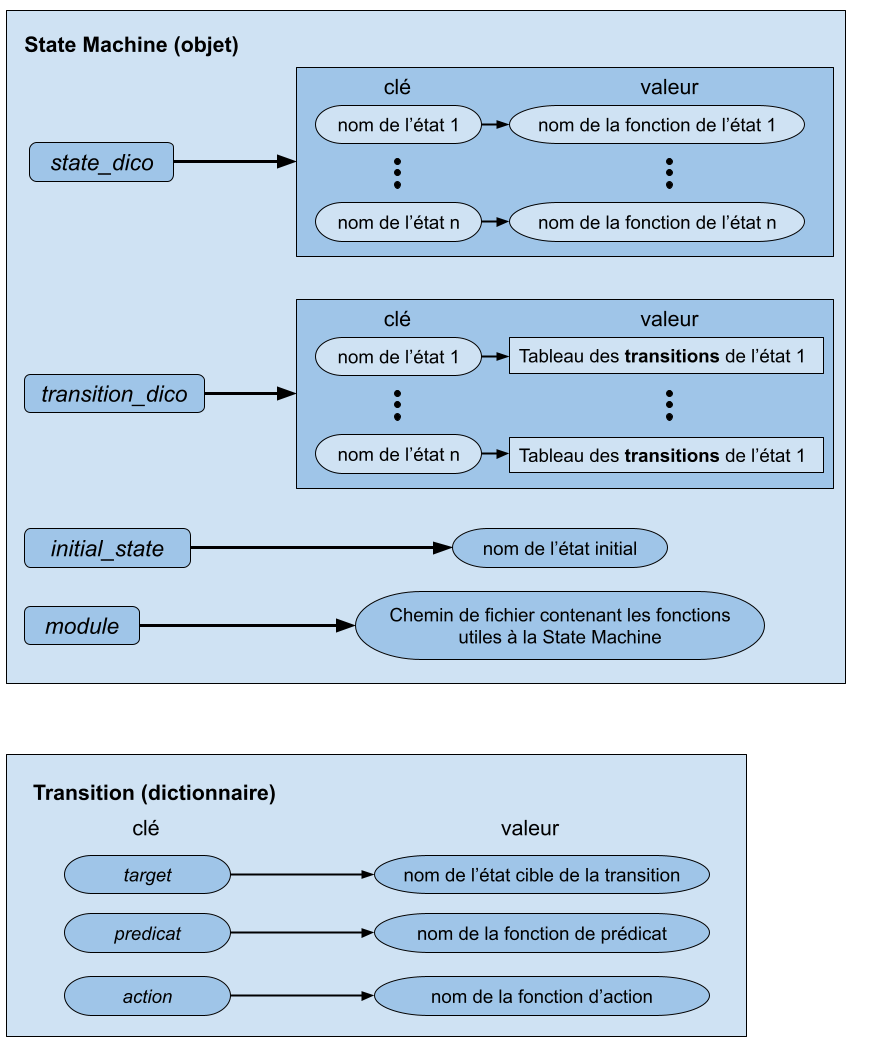
\includegraphics[scale=0.45]{figures/State_Machine.png}
    \caption{Schématisation de la State\_Machine}
    \label{fig:statemachine}
\end{figure}

Nous voyons donc que seule la State\_Machine est une classe à proprement parler tandis que les états et les transitions sont gérés par des dictionnaires et des tableaux. Dans ces différentes structures de données sont stockées des chaînes de caractères, il s'agit pour la plupart de noms de fonction qui sont ensuite appelées grâce à la fonction \texttt{getattr} de \texttt{Python}. Cependant, cette dernière a pour but de récupérer une fonction depuis une chaîne de caractères à l'intérieur d'un contexte. Or, la State\_Machine ne possède pas encore les fonctions qu'elle va utiliser c'est pourquoi elle est munie d'un attribut \texttt{module} qui représente le nom du fichier dans lequel sont implémentées les fonctions utilisées par la State\_Machine. Enfin, on trouve le champ \texttt{initial\_state} qui est simplement le nom de l'état initial de la State\_Machine. \\

Cela n'est pas directement mentionné dans le schéma mais la State\_Machine embarque une \texttt{Session} afin de pouvoir interagir avec le Reachy. Cette notion de \texttt{Session} est discutée plus en détail dans la Partie \ref{section_session}. 

\subsubsection{Notion d'exécuteur}

Une State\_Machine comme présentée jusqu'à présent est un objet composé d'états et de transitions. Cependant, elle n'est pas faite pour être exécutée directement par elle-même, il s'agit davantage d'une structure de données qui englobe les états et les transitions. Pour cela nous avons ajouté une notion d'exécuteur, au départ un exécuteur prenait en argument une machine à états et l'exécutait mais suite à une discussion avec M. Morandat nous avons décidé d'une solution plus logique. La State\_Machine est alors capable via une fonction, de se créer un exécuteur. Celui-ci est représenté par la classe \texttt{Executor} et son but est de partir de l'état initial de la machine, de l'exécuter, de regarder les prédicats des différentes transitions sortantes de cet état afin d'en emprunter une jusqu'à l'état suivant et ainsi de suite. C'est donc l'objet qui va parcourir la State\_Machine et plus précisément il s'agit du programme principal de Reachy. Afin d'avoir accès aux différents états et transitions, l'\texttt{Executor} possède un attribut enregistrant la machine à états qui l'a créé. Ainsi il l'utilise comme une structure de données afin de connaître les états, les fonctions associées, les transitions sortantes de chacun, etc...\\

L'un des principaux problèmes auxquels nous avons été confrontés afin de généraliser la machine à états a été le contexte d'exécution. En effet, une machine à états est un enchaînement d'états / transitions mais certaines valeurs doivent subsister aux états comme par exemple la \texttt{Session} qui est primordiale. C'est pourquoi nous avons ajouté un attribut à l'\texttt{Executor} nommé \texttt{context}. Il s'agit d'un dictionnaire, il est utilisé dans le fichier pointé par l'attribut \texttt{module} de la \texttt{State\_Machine} dans lequel chaque fonction, dès lors qu'elle veut faire transiter de l'information au-delà de son propre environnement, place sa valeur dans le dictionnaire \texttt{context} à une certaine clé. Ainsi une fonction d'un autre état saura la retrouver en allant simplement accéder au dictionnaire \texttt{context}.

\subsubsection{Fichiers JSON} \label{subsubsec:json}

Maintenant que nous avions généralisé la notion de machine à états, il a fallu trouver un moyen pour la création de ces objets State\_Machine. Il aurait été possible de créer à la main les différents dictionnaires et tableaux dans un fichier. Cependant, cela paraissait peu pertinent puisque cela oblige les personnes souhaitant créer une State\_Machine à connaître la structure en détail. Le choix s'est donc porté sur un stockage dans des fichiers \texttt{.json} et la création d'une fonction de chargement de ces fichiers pour les transformer en State\_Machine. Nous avons choisi les \texttt{.json} tout d'abord car ils se portent bien à notre problème étant donné qu'il est facile de représenter des dictionnaires et des tableaux dans ce type de fichier. De plus, en \texttt{Python} il est d'autant plus simple de lire un fichier \texttt{.json} car une fonction existe pour le transformer directement en structure de données \texttt{Python}. La fonction de chargement, \texttt{loader}, se base donc sur cette fonction de \texttt{Python} afin de dégager du fichier \texttt{.json} le dictionnaire d'états, celui de transitions,etc... Ensuite la fonction construit une State\_Machine à partir de cela et la renvoie. La Figure \ref{fig:json} illustre la structure du \texttt{.json} dont un exemple est présent en Annexe (cf \ref{subsec:annexe_json}).

\begin{figure}[H]
    \centering
    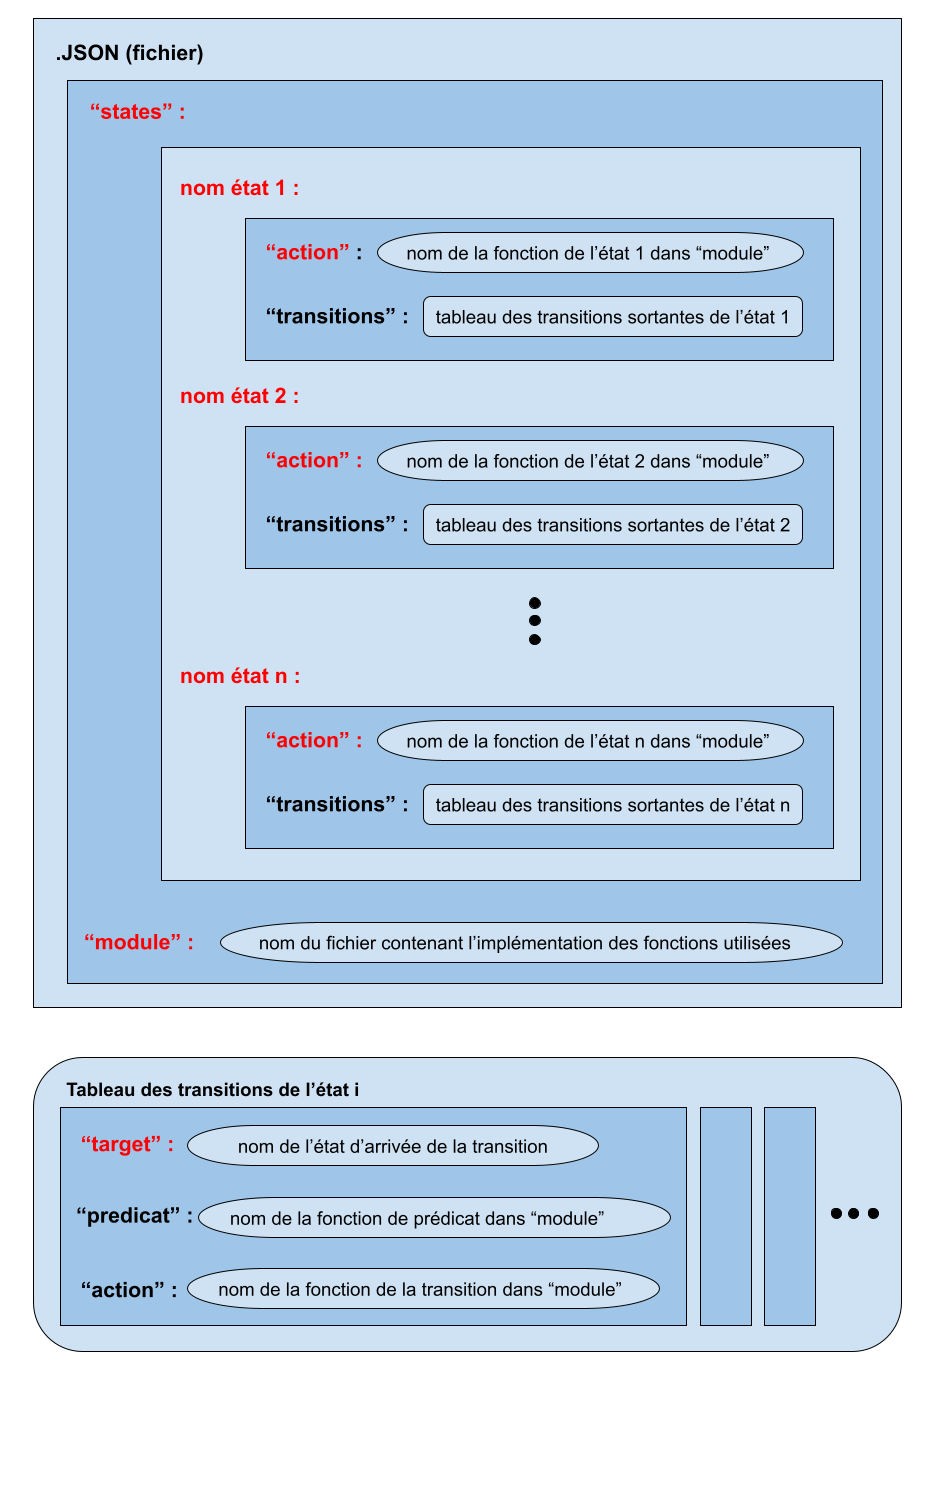
\includegraphics[scale=0.4]{figures/schema_JSON.png}
    \caption{Schématisation du format des fichiers \texttt{.json}}
    \label{fig:json}
\end{figure}

Nous remarquons donc sur la figure \ref{fig:json} que le format du fichier \texttt{.json} correspond plus ou moins à la structure de la machine à états. Néanmoins sur le schéma toutes les clés des dictionnaires ne sont pas toutes obligatoires et sont remplacées ensuite par l'\texttt{Executor} lors de l'exécution de la machine à états. Il s'agit des noms qui ne sont pas en rouge, ceux-ci sont obligatoires. Nous avons par exemple le prédicat d'une transition qui est facultatif et qui sera remplacé à l'exécution par une fonction qui renvoie toujours vrai. Nous pouvons donc assimiler cela à une transition par défaut. Il est important de noter que lors de la vérification des prédicats par l'\texttt{Executor}, celui-ci les vérifie dans l'ordre du tableau qui est le même que l'ordre dans le fichier \texttt{.json}. De ce fait, une transition dite par défaut par son absence de prédicat devra être placée à la fin du tableau pour ne pas rendre d'autres transitions inaccessibles. De plus, d'autres clés sont optionnelles comme l'action d'une transition qui sera remplacée par une fonction ne faisant rien. Enfin, on trouve le tableau de transitions en clé optionnelle, un état dépourvu de transition sera considéré comme état final et arrêtera l'exécution de la machine à états.

\subsubsection{Notion de Timeout pour un état}

Après la généralisation de la machine à états, nous avons essayé de mettre en place une première machine de test pour le Reachy. La \texttt{State\_Machine} de celui-ci comporte des \texttt{timeout} sur certains états qui obligent à changer d'état au bout d'un certain nombre de secondes. La première implémentation de cela s'est faite via des transitions dans la machine à états avec une fonction de prédicat qui vérifie le temps passé depuis le début de l'état (valeur sauvegardée dans le contexte). Si cette durée était supérieure  à une certaine valeur alors la transition était prise. Cependant, cette méthode rend plus difficile l'écriture du fichier \texttt{.json} et de plus, chaque fois qu'un nouveau timeout devait être fait avec une durée en secondes différentes il fallait créer un prédicat différent ce qui n'est pas pratique lorsque plus de 3 ou 4 états ont besoin de ce système. Ce qui a été décidé pour régler ce problème est l'ajout d'une clé optionnelle \texttt{"timeout"} dans chaque état du fichier \texttt{.json}. La figure \ref{fig:timeout} schématise cet ajout.

\begin{figure}[H]
    \centering
    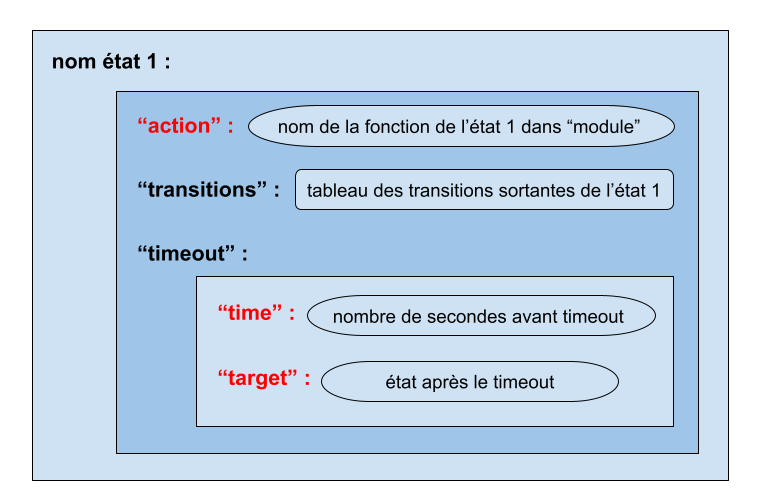
\includegraphics[scale=0.4]{figures/schema_timeout.png}
    \caption{Schématisation du format des timeouts dans les \texttt{JSON}}
    \label{fig:timeout}
\end{figure}

Nous pouvons voir sur la figure \ref{fig:timeout} que la clé \texttt{"timeout"} est optionnelle, si elle n'est pas renseignée l'exécuteur continuera à boucler sur l'état tant que celui-ci n'a pas de prédicat de transition vérifié. \texttt{"timeout"} est un dictionnaire composé de 2 clés, \texttt{"time"} qui est un entier représentant le nombre de secondes avant le timeout et \texttt{"target"} qui est l'état à atteindre en cas de timeout. \\

Cet ajout a fortement facilité l'implémentation de timeouts et de la machine à états en général qui pouvait devenir compliquée avec la gestion du temps depuis l'arrivée dans un état et tout ce que cela implique comme la réinitialisation du temps dans le contexte par des actions de transitions.

\subsubsection{Lancer une machine à états sur le Reachy}

Afin de lancer une machine à états sur le Reachy il suffit simplement de lancer un exécuteur de la \texttt{State\_Machine} choisie puisque Reachy peut être assimilé à un exécuteur. Pour cela il faut créer une session (cf Partie \ref{section_session}), la donner à l'exécuteur et lancer ce dernier. Le Reachy va alors passer d'états en états en effectuant les actions associées. \\

Après la généralisation de la notion de machine à états, pour chaque \texttt{State\_Machine} un fichier \texttt{Python} était créé afin de charger la machine, créer une session et lancer un exécuteur sur celle-ci. Cela commençait à prendre de la place et surtout à rendre illisible le fichier \texttt{src/state\_machine}. C'est pourquoi nous avons implémenté un fichier qui utilise la ligne de commande pour charger le fichier \texttt{.json} voulu. Il en existe 2, les deux prennent en argument le chemin relatif vers la machine à états  au format \texttt{.json} (cf Partie \ref{subsubsec:json}), la charge et l'exécute. Cependant, l'un le fait avec une session associée au Reachy tandis que l'autre le fait avec une fausse session afin de pouvoir tester les machines à états sans avoir besoin de se déplacer au FabLab. \\

En conclusion de cette partie sur la machine à états, sa généralisation nous a pris beaucoup plus de temps que la première implémentation cependant nous avons pu ensuite gagner énormément de temps. Nous avons même pu en quelques minutes préparer des \texttt{State\_Machine} de tests et en 1 heure il a été possible d'écrire une machine à états pour la soirée partenaire avec l'utilisation exclusive de codes ARUCO.

\section{Les différentes fonctionnalités}
Pour permettre au robot d'interagir avec les utilisateurs, il fallait tout d'abord rendre possible la reconnaissance vocale.
\subsection{Reconnaissance vocale}

Toute la partie reconnaissance vocale a été implémentée grâce aux bibliothèques \texttt{PyAudio} pour la récupération du son ainsi que de \texttt{speech\_recognition} pour la partie traduction de vocal à texte. Cela correspond au cahier des charges.

\subsubsection{Gestion des mots-clé}    
La partie reconnaissance vocale devait dans un premier temps être capable de reconnaître des mots-clés et de réagir en fonction. Pour la partie ordre, la reconnaissance d'un mot-clé doit déclencher un changement d'état et cela est vérifié par les prédicats présentés dans la partie \ref{subsubsec:StMaGeneral}. Pour la partie conversation, la reconnaissance des mots-clés se traduit par un ensemble de mots d'entrée qui donnent lieu à des mots-clés de sortie. Cela a été mis en place grâce à des fichiers \texttt{.txt} comportant, comme spécifié dans le cahier des charges, un ensemble de mots de sortie et un ensemble de mots d'entrée. Dans un fichier \texttt{Python} nous avons implémenté des fonctions qui ouvrent ces fichiers et en créer des tableaux avec l'ensemble des mots-clés. Ensuite, dans la machine à états, il y a une comparaison entre le texte obtenu par la fonction de reconnaissance vocale et les tableaux afin de savoir quels mots sont présents et en déduire une sortie. Un principe similaire a été appliqué pour les mots-clé donnant lieu à un changement d'état. La Figure \ref{fig:keywords} schématise les différents éléments qui entrent en jeu dans le système de reconnaissance vocale. 

\begin{figure}[H]
    \centering
    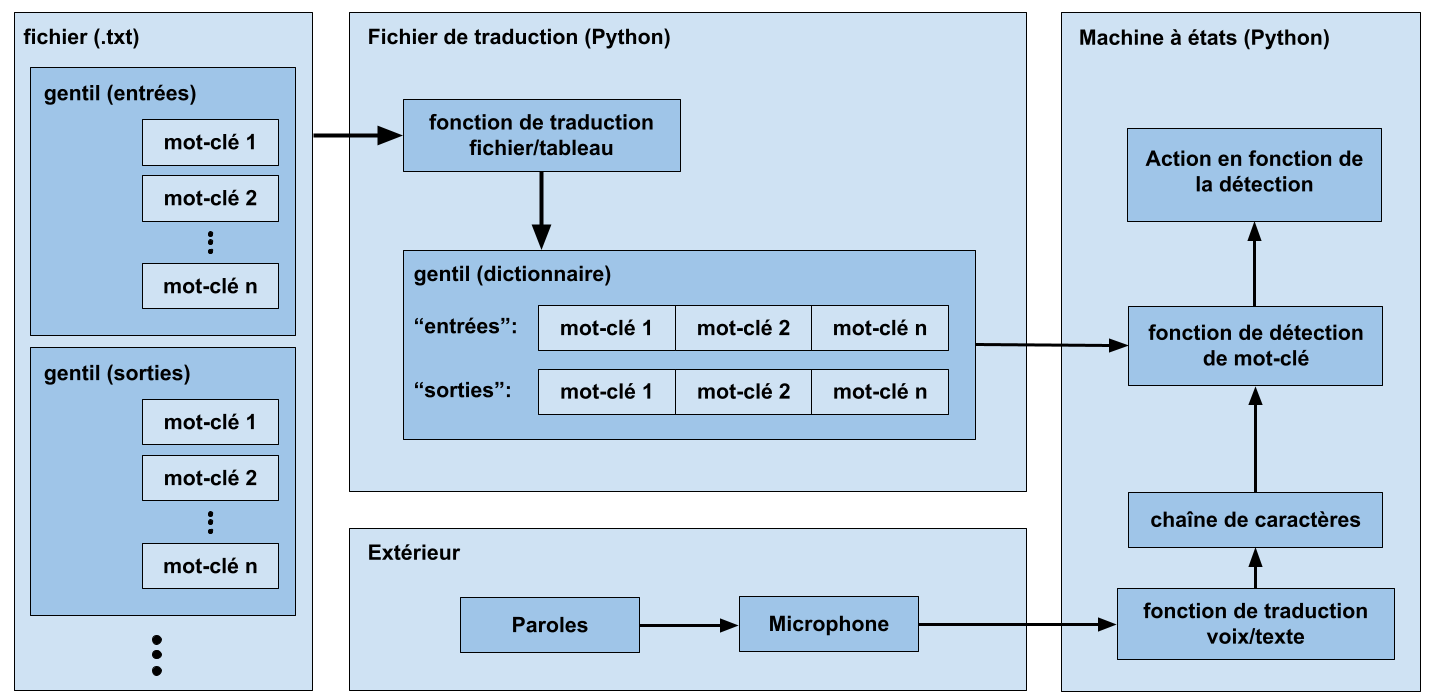
\includegraphics[scale=0.35]{figures/keywords.png}
    \caption{Schématisation des étapes de la reconnaissances de mots-clé pour le conversation}
    \label{fig:keywords}
\end{figure}

Nous remarquons sur la figure \ref{fig:keywords} que les entrées et sorties des conversations sont gérées par des dictionnaires ce qui rend l'utilisation des couples entrée/sortie plus simple. \\

Toutes ces interactions entre fichiers, fonctions de traduction et machine à états viennent d'une réflexion afin de rendre l'utilisation de mots-clés plus accessibles. En effet, de cette manière pour ajouter un mot-clé à un couple entrée/sortie ou bien un mot-clé pour passer de l'état \texttt{Attente d'ordre} à \texttt{Photo} par exemple, il suffit simplement à l'utilisateur d'ajouter un mot dans un fichier texte sans toucher au code. Cela paraissait beaucoup plus instinctif. Cependant, si l'utilisateur souhaite créer un nouvel ensemble de mots-clés il est obligé d'effectuer quelques modifications dans le code. Au moins pour le système d'entrée/sortie, il aurait été intéressant d'automatiser tout ce processus pour permettre à l'utilisateur d'ajouter des couples d'entrée/sortie sans toucher à une seule ligne d'un fichier \texttt{Python}. Cela aurait également permis de factoriser du code mais on aurait perdu le fait d'ajouter des mouvements de réaction aux mots-clés pour le Reachy. La solution actuelle semble donc convenir dans la mesure où les modifications sont minimes et que l'on gagne en logique dans la machine à états. 

\subsubsection{Gestion prise du son}
Afin d'enregistrer la voix de l'interlocuteur avec le robot nous avons utilisé le microphone interne à celui-ci. Cependant nous n'avons pas réussi à trouver des réglages convenables, il fallait donc la plupart du temps parler très fort et lorsqu'il y avait du son parasite il était impossible de lui faire détecter des mots-clé. Même avec l'utilisation de fonctions de réduction du bruit, il était impossible d'obtenir un résultat convenable. Nous avons essayé de changer de microphone en lui branchant le même modèle que son micro interne mais cette fois-ci à l'extérieur mais le problème était le même. Le problème venait donc du modèle du microphone et non pas du microphone interne en particulier. Nous avons ensuite essayé avec un casque-micro et cette fois-ci aucun problème de compréhension même dans un environnement moyennement bruyant. La solution que nous avons trouvée est donc d'utiliser le micro du casque-micro pour l'entrée audio et les hauts-parleurs du Reachy pour la sortie audio. 

\subsubsection{Réduction du bruit}

Pour ce qui est de la réduction du bruit, il était mentionné dans le cahier des charges que nous devions utiliser un système afin d'obtenir une entrée avec des bruits parasites réduits pour le Reachy. Nous avons réalisé cela grâce à une bibliothèque \texttt{Python} et après les tests avec le casque-micro cela fonctionne correctement. Afin de vérifier ce bon fonctionnement nous sommes passés par des sous-fichiers, c'est-à-dire que nous enregistrions la voix brute dans un premier fichier puis nous effectuons un traitement sur celui-ci et enregistrions le résultat dans un second fichier. Cela nous a permis de les comparer et nous avons observé une amélioration au niveau des bruits parasites. La figure \ref{fig:reduction} illustre cette variation, pour obtenir cette courbe nous nous sommes enregistrés disant une commande au Reachy dans des conditions de bruit relativement élevées. \\

\begin{figure}[!ht]
    \centering
    \begin{subfigure}{1\textwidth}
        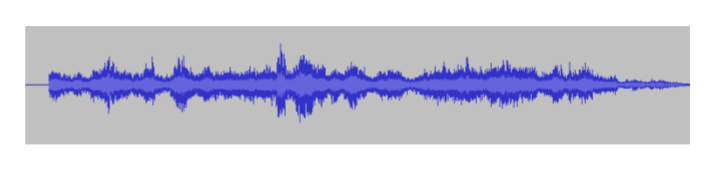
\includegraphics[width=\textwidth]{figures/sans_reduction.png}
        \caption{Sans réduction}
    \end{subfigure}
    \begin{subfigure}{1\textwidth}
        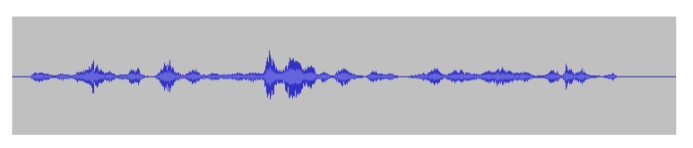
\includegraphics[width=\textwidth]{figures/avec_reduction.png}
        \caption{Avec réduction}
    \end{subfigure}
    \caption{Visualisation de la différence avec ou sans la fonction de réduction du bruit} 
    \label{fig:reduction}
\end{figure}

\subsubsection{Conversation avancée} 
Le robot doit être capable de mener une conversation soit du type simple ou du type avancée. Dans le cahier des charges, nous avons mentionné que la conversation avancée allait être implémentée de la même façon que la conversation simple, c'est-à-dire, en utilisant des mots-clés et en ajoutant  une notion de mémoire de l’état à la conversation. Nous nous sommes rendus compte, que la conversation allait rester toujours très limitée. Alors, nous avons décidé d'utiliser \texttt{OpenAI}.\\
\texttt{OpenAI} est une API qui permet d'accéder à \texttt{GPT-3} une intelligence artificielle qui effectue diverses fonctionnalités du traitement du langage naturel ( ou en anglais Natural Language Programming NLP). Il y a quatre modèles (ou engines) dans \texttt{GPT-3} : \texttt{"text-davinci-002"}, \texttt{"text-curie-001"}, \texttt{"text-babbage-001"} et \texttt{"text-ada-001"}. Chacun de ces modèles a des caractéristiques et des niveaux de performances destinées à des tâches spécifiques. Nous avons choisi \texttt{"davinci"} parce qu'il est le modèle le plus puissant et parce que l'API est en version \texttt{beta}. \\
Ainsi, pour utiliser cela, nous avons dû fixer quelques paramètres:

\begin{itemize}
    \item température: La température est un paramètre qui permet de contrôler la diversité des réponses et qui donne un effet de l'aléatoire. Il est compris entre 0 et 1. Plus on s'approche de zéro, plus les réponses sont déterministes et répétitives. Choix : 0.9
    \item max\_tokens: est le paramètre qui fixe la taille en nombre de mots de la réponse en sortie. Nous l'avons fixé à 100 pour que le robot ne donne pas des réponses trop longues et ennuyeuses pour l'utilisateur.
    \item best\_of: L'algorithme génère, pour chaque entrée, plusieurs réponses avec une certaine probabilité. Ce paramètre permet de fixer le nombre des meilleures sorties (nous avons choisi de le mettre à 1) pour avoir seulement la réponse avec la plus grande probabilité.
    \item top\_p: La probabilité utilisée pour filtrer les réponses. Si elle est à 50\% , alors la moitié de toutes les options pondérées probables sont considérées pour filtrer la réponse. (choix: 1)
    \item frequency\_penalty: permet de pénaliser les nouveaux "tokens" ou mots en se basant sur leur fréquence de présence dans la conversation. Cela permet d'éviter la répétition. (choix : 0)
    \item presence\_penalty: permet de pénaliser les nouveaux tokens s'ils ont apparu dans la conversation. Cela permet d'encourager le modèle à parler de nouveaux sujets. (choix : 0.6)
\end{itemize}

Après l'intégration de cette fonctionnalité, nous avons rencontré un problème de langues. En effet, \texttt{GPT-3} est censé parler en anglais comme langue par défaut. Et puisque le choix de la voix était en français, c'était très difficile de comprendre les réponses du robot. Et d'une manière générale, le fait d'avoir des entrées dans une langue et la sortie dans une autre langue diminue nettement la performance.
La solution initiale que nous avions trouvée est l'ajout de certaines phrases d'initialisation écrites en français pour le forcer en quelque sorte à parler en français. Mais après l'ajout de l'état incompréhension "qui mène vers la conversation avancée", nous avons décidé de lui passer en paramètre un \texttt{context} qui lui permet d'enregistrer l'état de la conversation avec l'utilisateur avant le début de la conversation avec l'IA et donc d'initialiser une conversation en français dans ce \texttt{context}.


\subsection{Synthèse vocale}
L'une des fonctionnalités de Reachy requise dans le cahier des charges est de parler et d'interagir avec l'utilisateur. Tout le code de la partie synthèse vocale est présent dans le répertoire \texttt{speech} de \texttt{src}. Il est séparé en deux fichiers principaux. Le fichier \texttt{speech\_synthesis.py} qui implémente une première utilisation de la bibliothèque Python \texttt{pytttsx3}. Un deuxième fichier \texttt{speech\_synthesis\_gtt.py} qui lui implémente la solution maintenue qui repose sur l'utilisation de l'API \texttt{gTTS}.

\subsubsection{Utilisation de pyttsx3}
Le module \texttt{pyttsx3} est une bibliothèque de conversion de texte en parole en Python\ref{fig:syntheseVocale}. Sa particularité principale est son fonctionnement hors ligne. Il supporte deux voix: la première est féminine et la seconde est masculine. Il prend en charge 3 moteurs TTS: \texttt{sapi5}, \texttt{nsss} et \texttt{espeak}. Nous avons utilisé le moteur espeak, comme indiqué dans le cahier des charges, vu que les deux autres moteurs TTS ne peuvent pas être lancés et ne sont pas pris en charge sous Linux.\\

\begin{figure}[H]
    \centering
    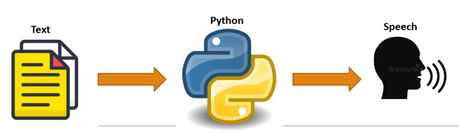
\includegraphics[scale=0.8]{figures/synthese_vocal.png}
    \caption{Synthèse vocale}
    \label{fig:syntheseVocale}
\end{figure}

Tout le code qui utilise le module \texttt{pyttsx3} a été implémenté dans le fichier \texttt{speech\_synthesis.py} du répertoire \texttt{speech}. On y contrôle directement le volume, la vitesse et la voix.\\
Cependant, malgré le bon fonctionnement du code, la voix générée reste très mécanique. Et ceci s'explique par le fait que nous utilisons le synthétiseur vocal espeak. La seule option pour améliorer et changer la voix générée par le module \texttt{pyttx3} était de sélectionner l'un des deux autres moteurs TTS. Cepedant, ceci était impossible à réaliser puisque les deux autres synthétiseurs ne sont pas prises en charge sous Linux.

\subsubsection{Utilisation de gTTS}
Une des solutions que nous avons envisagée pour avoir une voix robotique mais pas trop mécanique est d'utiliser un autre module de synthèse vocale. C'est pourquoi nous avons choisi d'utiliser le module \texttt{gTTS}, Google Test-to-Speech, qui utilise l'API de synthèse vocale de Google Traduction. Cet outil est en ligne est nécessite donc un accès à Internet. Ce moteur propose une voix féminine et non modifiable. Néanmoins, nous avons trouvé que la voix proposée n'est ni humaine, ni très mécanique. Elle correspond parfaitement à la voix d'un petit robot.\\

\begin{figure}[H]
    \centering
    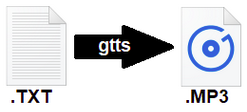
\includegraphics[scale=0.8]{figures/gtts.png}
    \caption{\texttt{gTTS} pour la conversion d'un texte en audio}
    \label{fig:gTTS}
\end{figure}

L'API propose différentes langues pour la lecture du texte en entrée. Nous avons décidé de fixer ce paramètre et de choisir le Français comme langue de communication entre l'utilisateur et le robot.\\

\textbf{Déroulement du script:} 
À l'exécution du script, la fonction \texttt{text\_to\_speech} prend en entrée un texte, génère la voix associée dans un fichier \texttt{.mp3} temporaire dans le répertoire \texttt{tmp/}, lit le fichier et le supprime directement après pour optimiser l'espace mémoire. À la lecture du fichier, le son sort directement de la sortie audio du robot.\\

\textbf{Transcription d'une émotion ou d'un état:}
Il a été spécifié dans le cahier des charges d'émettre des sons et des bruits suivant les émotions et les états du robot. Pour ce faire, différents sons ont été mis dans le dossier \texttt{voices/} sous forme de fichiers \texttt{.mp3}, et chaque son est émis suivant l'état du robot, lorsqu'il prend une photo par exemple, il compte jusqu'à trois et émet un son de flash, comme si la photo était prise par un appareil photo.\\

\textbf{Structuration du code:} 
Pour certains états et transitions de notre machine à états,  le robot doit émettre du son, soit pour communiquer avec l'utilisateur ou pour exprimer ses émotions via de petits bruits. Pour cela, nous avons consacré une fonction pour chaque état ou transition, ayant besoin de la synthèse vocale, pour sélectionner le son associé. \\

\textbf{Amélioration possibles:} 
\begin{itemize}
    \item Nous pouvons imaginer un système qui vérifie si le robot est connecté à internet ou pas. La réponse renvoyée décidera si le robot utilisera la version connectée \texttt{gTTS} ou la non connectée \texttt{pyttsx3}.
    \item Une deuxième amélioration possible serait de laisser la possibilité à l'utilisateur de configurer la langue avec laquelle il aimerait interagir avec Reachy.
\end{itemize}

\subsection{Traitement d'image}
L'une des grandes fonctionnalités de Reachy requise par le client est la capacité à prendre des photos "bien" cadrées, ainsi que d'apporter certaines retouches aux photos prises mais aussi de suivre une personne du regard pour rendre l'interaction plus naturelle. Pour ce faire et respecter les contraintes fonctionnelles, nous devions implémenter la capacité d'identifier des visages (au sens de la détection) et de cadrer les personnes souhaitant être prises en photo, avant de considérer l'ajout de filtres sur les photos en questions.\\

Ces services sont implémentés dans le fichier \texttt{face\_detection.py}. L'architecture de ce code source a été pensée de façon modulaire en offrant une interface pour le recours aux dits services, mais est également pensée de façon fonctionnelle et en couche \footnote{Les couches sont : transformations mathématiques en espace plan, traitement de tableaux, sous fonctions offrants des traitements paramétrables à l'interface, fonctions d'interaction avec les sessions, fonctions faisant office d'interface}. Ces propriétés permettent une maintenance et une amélioration facile du code en plus de permettre la composition de plusieurs services afin d'offrir une explosion combinatoire de transformations d'images.

\subsubsection{Prise de photos}
\textbf{Détection de visages}\\

La première problématique a été l'intégration de la capacité à détecter des visages. La détection faciale étant une branche importante de l'intelligence artificielle, la méthode la plus efficace pour recourir à un algorithme performant consista à exploiter une bibliothèque implémentant des services de vision par ordinateur.\\

\textbf{OpenCV} est une bibliothèque proposant de nombreuses fonctionnalités de vision par ordinateur et spécialisée dans le traitement d'images en temps réel. C'est une bibliothèque très médiatisée, facile d'utilisation et que certains membres de l'équipe ont déjà manipulée. Celle-ci nous a permis d'économiser du temps sur les détails techniques de l'implémentation des méthodes permettant de fournir les services requis. Qui-plus-est, cette bibliothèque nous a été conseillée par le client pour ces mêmes raisons pratiques.\\

\textbf{Le port du masque}\\

La première implémentation consista en une interface exploitant l'une des caméras \footnote{Nous aborderons dans la suite la raison d'un tel choix} de Reachy pour identifier des visages dans son champ de vision et proposer des angles de rotation en repère sphérique à l'interface de mouvement afin d'obtenir une première approche du suivi de visage et d'un cadrage. Le problème majeur inattendu lors de la programmation et tests à distance de cette implémentation fut la présence de masques contre la COVID-19. Ceux-ci cachaient une partie conséquente des visages ce qui entravait les capacités de détection de visages de certaines méthodes cherchant la présence d'un nez et d'une bouche pour fonctionner. Cette découverte lors d'un test au Fablab a restreint la gamme de méthodes de reconnaissance faciale utilisables.\\

En conséquence, la méthode la plus connue et résistante au port du masque est la \textbf{classification en cascade de Haar}. Grâce à des fenêtres de détection \footnote{Ce sont des matrices parcourant une image afin d'associer des valeurs à des portions de l'image pour identifier des schémas particuliers} permettant d'analyser localement la répartition des couleurs sur une image, la méthode de Viola et Jones exploitée dans cette classification en cascade permet de reconnaître de nombreux objets et formes. Cette propriété permet, en possession d'un classificateur entraîné, de reconnaître uniquement la partie frontale d'un visage. Ceci nous a permis de recourir à une méthode fonctionnant avec ou sans port du masque grâce à la détection des yeux et du front en tant que détection faciale. Ce problème n'a pas été handicapant étant donné la modularité de la bibliothèque \textbf{OpenCV} permettant aisément de changer de méthode de reconnaissance faciale au sein du code source. \\

\textbf{Tangage de la tête}\\

Un problème paraissant en tant que dette technique fut la difficulté avec laquelle la tête de Reachy se mouvait sans induire un penchement de la tête. Ce problème de tangage fut corrigé par les membres de l'équipe gérant les mouvements. Cependant, sans une telle correction, l'analyse d'image en vu de fournir des angles de déplacement de la tête aurait été mise en défaut.\\

Le problème venait de l'interprétation qu'avait Reachy de son environnement visuel. Avec une tête penchée comme montré en figure \ref{fig:Tangage}, Reachy conçoit les axes vertical et horizontal selon le référentiel de sa caméra. Or, avec une tête penchée, ce référentiel n'est plus confondu avec celui de la salle formant son environnement. Cette déformation visuelle nous a empêché d'effectuer des tests corrects de suivi de visages et de cadrage de photos. Cela s'explique par le fait que les angles de déplacement offerts par l'interface de vision par ordinateur étaient penchés par rapport à ceux que l'interface de mouvement utilise (fidèles au repère de l'environnement).

\begin{figure}[H]
    \centering
    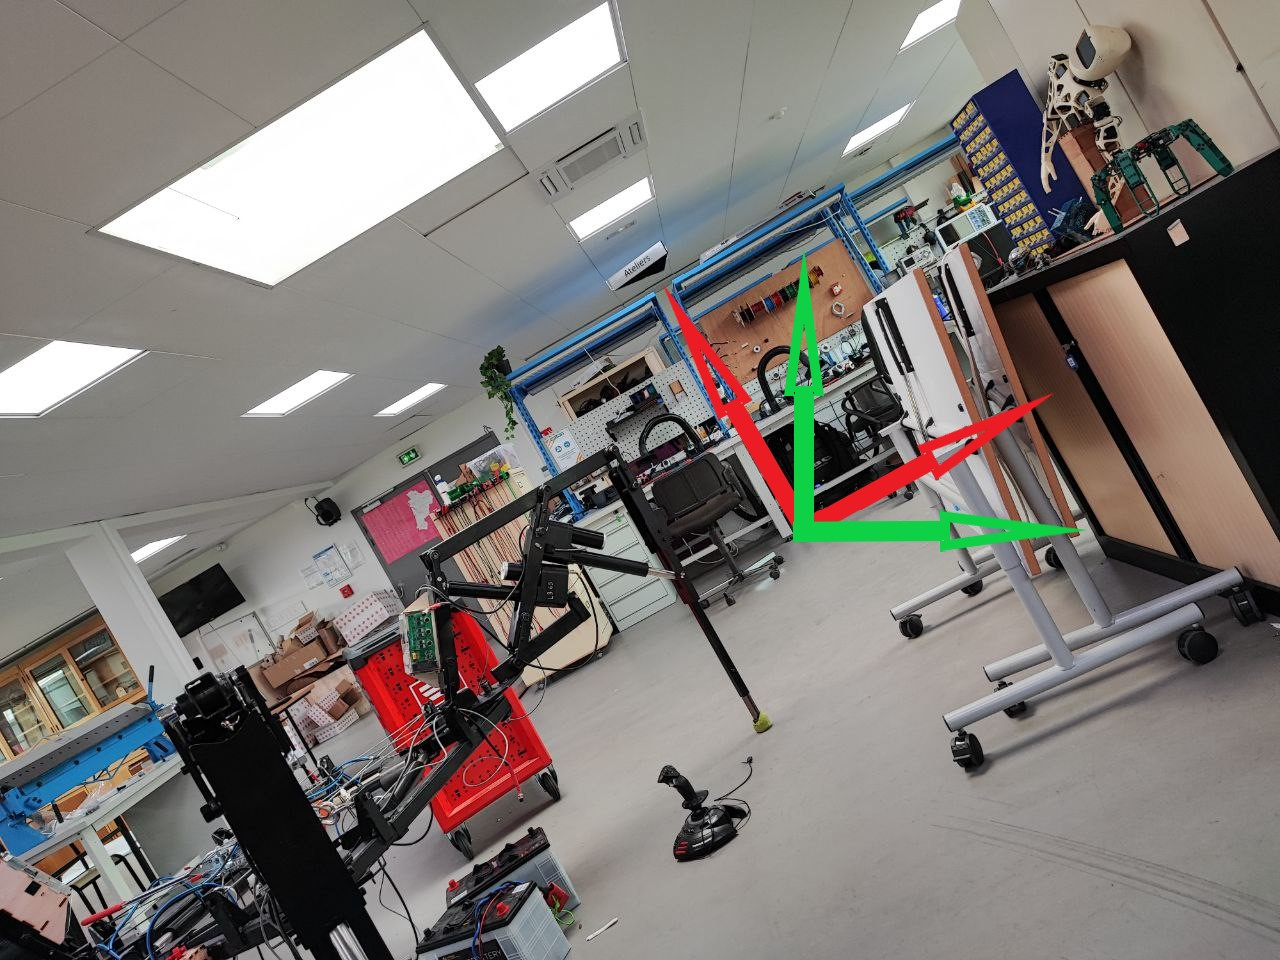
\includegraphics[scale=0.27]{figures/tangage.jpg}
    \caption{Exemple de décalage entre les référentiels rouge (de la salle) et vert (de la caméra)}
    \label{fig:Tangage}
\end{figure}

Avant la découverte d'une correction de ce problème au niveau de l'interface de mouvement, nous avons conçu diverses stratégies inefficaces ayant pour objectif d'offrir une correction au niveau de l'analyse d'image même.\\
La première fut l'exploitation de capteurs propres à Reachy permettant d'avoir une connaissance du tangage de la tête pour apporter une rectification des angles de mouvement au travers d'une transformation de ceux-ci. Cependant, la manipulation des moteurs étant très bas niveau, cette solution n'a pas été retenue pour sa complexité de développement.\\
La seconde alternative aurait été l'analyse d'une ligne d'horizon dans l'image même afin de déterminer le tangage et d'apporter les corrections d'angles. Mais Reachy étant posé sur une table, celui-ci voit son champ de vision souvent en contre-plongée, empêchant ainsi de voir le sol qui aurait servi à définir l'horizon. La rectification dans l'interface du mouvement a été apportée assez rapidement pour que nous n'explorions pas d'autres pistes de correction.\\

\textbf{Une ou deux caméra(s) ?}\\

Une nouvelle entrave au suivi de visages était dans le recours à une caméra en particulier. En effet, Reachy possède deux caméras d'avantages espacées que des yeux humains. Nous avions une appréhension quant à la façon avec laquelle Reachy regarderait un individu.\\
Ainsi, nous avions pensé à utiliser une méthode de transformation linéaire afin de coupler la vision des deux caméras en une seule image pour prôner la cohérence avec laquelle Reachy fixerait quelqu'un. Ceci n'étant pas problématique pour le cadrage de photo, et étant donné que la caméra regardant de face un individu est celle prenant les photos, le client et nous-même n'avons pas jugé pertinent de consacrer du temps à une telle correction. De plus, lors de nos premiers tests de suivit de visages, la façon dont le robot ciblait une personne du regard était tout à fait naturelle. \\

\textbf{Cadrage}\\

Concernant le cadrage des photos selon les visages à capturer, celui-ci se décompose en deux catégories. La première est le cadrage d'une photo simple, c'est-à-dire une photo ne comprenant qu'une seule personne, tandis que le second type concerne la prise de photos de groupe.\\

Après connaissance du type de photo à effectuer, le robot ajuste la position de sa tête en conséquence afin de cadrer la photo. Dans le cas particulier d'une personne seule, nous avons convenu avec le client qu'il est naturel de centrer la photo sur le centre du visage de la personne concernée comme montré en figure \ref{fig:Bary_solo}. Afin de s'assurer que d'autres visages n'interfèrent pas avec celui de la personne à cadrer, un traitement de l'image identifie le visage le plus proche de Reachy et considère ce visage comme étant celui de l'utilisateur actuel. Cette politique a été approuvée par le client.\\

Cependant, la notion de proximité est complexe dans le domaine de la vision par ordinateur. Des méthodes recourant à de l'intelligence artificielle permettent d'avoir une estimation de la distance d'un visage à la caméra mais ces méthodes sont très versatiles selon la luminosité et la présence d'obstacles à proximité du visage induisant une distorsion des distance parasitant la distance prédite. Nous avons donc choisi, avec l'accord du client, d'approximer la notion de distance à la longueur d'un visage. Ceci permet de connaître une distance de façon déterministe et faiblement impactée par la différence de taille de visages.

\begin{figure}[H]
    \centering
    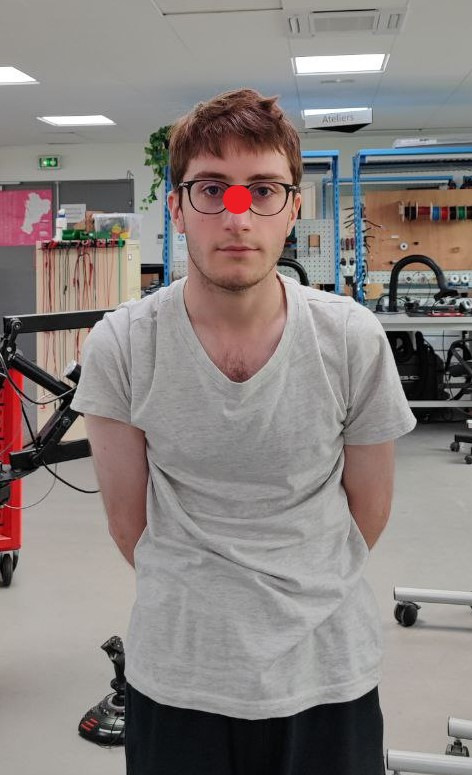
\includegraphics[scale=0.5]{figures/bary_solo.jpg}
    \caption{Placement du barycentre (point rouge) pour le cadrage d'une personne}
    \label{fig:Bary_solo}
\end{figure}

Le cas d'une photo de groupe demanda d'avantages de réflexion sur la façon d'éliminer les visages parasites mais aussi de cadrer d'une façon satisfaisante pour le client.\\

La politique d'élimination des visages parasites n'a pas reçu de contraintes venant du client. Une façon d'aborder ce souci s'est portée sur le recours à la proximité des visages \footnote{toujours approximée par la hauteur des visages}. Après identification de tous les visages dans le champ de vision de Reachy, une analyse de la proximité moyenne est effectuée. Avec une paramétrisation de l'écart à cette moyenne permise pour les visages présents, il nous a été possible d'éliminer les visages trop loin ou trop proches de cette moyenne, étant jugés comme n'appartenant pas au groupe \footnote{Considéré comme un ensemble de visages ayant une distance assez homogène à Reachy} qui représente la majorité des visages à prendre en compte, donc possédant la plus grande pondération dans le calcul de la moyenne. Avec plusieurs essais (facilités grâce à la paramétrisation), il nous a été possible de calibrer cette élimination de façon subjectivement satisfaisante.\\

Enfin, une fois les visages indésirables enlevés de l'ensemble à considérer, le cadrage peut être effectué sur l'échantillon de visages restants. La façon dont le cadrage de groupe est réalisé a demandé quelques échanges avec le client afin de choisir une façon parmi deux proposées.\\

La première façon était de considérer la même distance séparant le visage le plus à gauche de la limite gauche du champ de vision de Reachy de la distance entre le visage le plus à droite et la limite droite du champ de vision de Reachy. Cette méthode n'était pas concluante dans la mesure où une personne éloignée du groupe sur le côté du champ de vision de Reachy (mais à la même distance de Reachy que les membres du groupe à prendre en photo) aurait joué un rôle indésirable et trop important dans le cadrage.\\
La seconde approche a été approuvée par le client et ainsi retenue. Celle-ci consiste à calculer le barycentre des points incarnant les centres des visages à cadrer. De ce fait, le cas précédent d'une personne sur le côté sera en partie corrigé avec une préférence d'orientation de la tête vers la majorité. Le résultat d'un tel calcul est visible en figure \ref{fig:Bary_groupe}.\\

\begin{figure}[H]
    \centering
    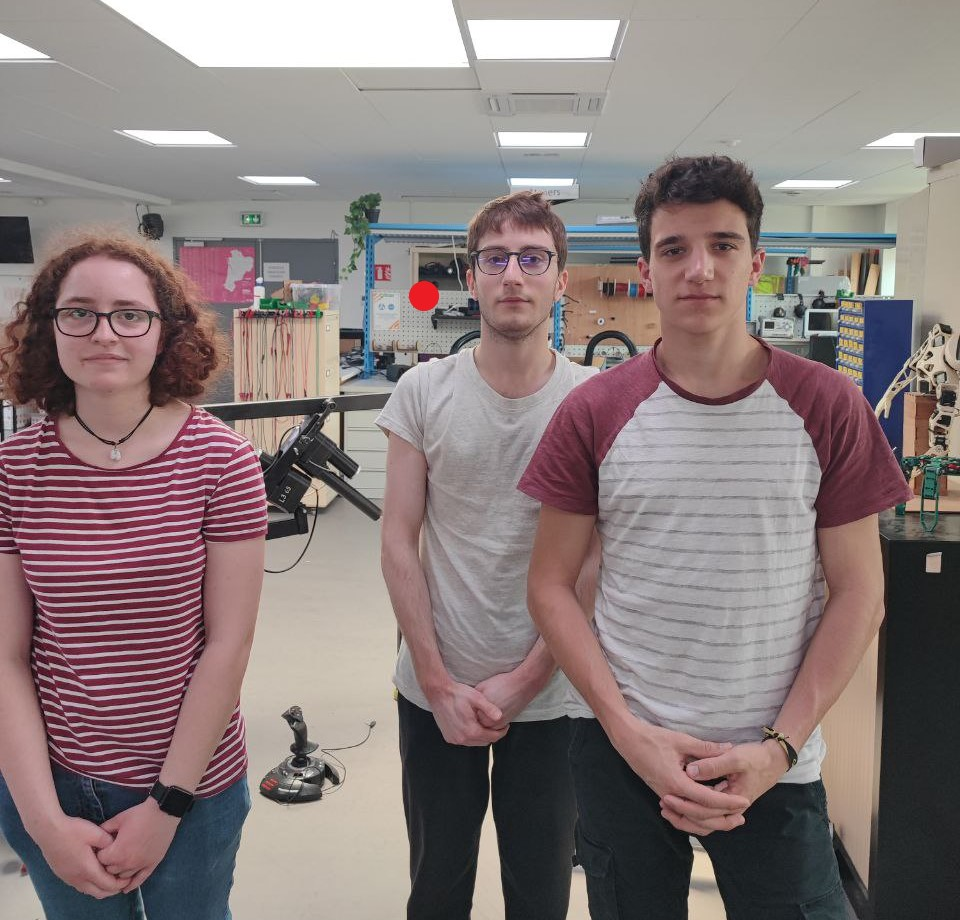
\includegraphics[scale=0.5]{figures/bary_groupe.jpg}
    \caption{Placement du barycentre (point rouge) pour le cadrage d'un groupe}
    \label{fig:Bary_groupe}
\end{figure}

\textbf{La mise au point}\\

Un problème handicapant la faculté visuelle de Reachy fut la gestion de la mise au point. Celle-ci peut être demandée via l'interface de Reachy mais la mise au point automatique était compliquée à maîtriser. Au départ, nous utilisions la mise au point avant chaque prise de photo afin que ladite photo soit nette. Or, l'échec de la mise au point rendait les photos floues. De plus, après échange avec le client, nous nous sommes rendu compte qu'une seule mise au point au lancement de Reachy était suffisante quelque soit la distance des personnes prises en photo par rapport à la caméra. Ainsi, afin de corriger le placement de la focale de la caméra dès que nécessaire, un programme est exécutable en parallèle de la machine à états. Ce programme affiche les images de la caméra en temps réel et lance la mise au point tant qu'une touche du clavier n'est pas pressée. Ceci permet de stopper la mise au point manuellement dès que les images envoyées par la caméra sont nettes.\\

Toutes les fonctionnalités concernant les manipulations visuelles de Reachy avant les 100 ans de l'Enseirb-Matmeca ont pu être implémentées fidèlement aux demandes du client répertoriées dans le cahier des charges.

\subsubsection{Filtres}
Deux filtres ont été proposés et retenus par le client. Le premier consiste à retirer les couleurs d'une photo afin de la proposer en noir et blanc. Le second filtre, requérant une étude plus poussée quant aux attentes du client, était d'effectuer un échange de visages.\\

La coloration en noir et blanc a été très rapide étant un service déjà fourni par la bibliothèque \textbf{OpenCV}.\\

L'échange de visages est une retouche d'image très médiatisée et appréciée du client. Différentes approches existent afin d'obtenir des résultats plus ou moins poussés. Afin de satisfaire le client, ayant affirmé sa satisfaction sur une échange basique de deux visages par 'copié-collé' directe des zones, une méthode avancée d'échange de visages a été implémentée, la \textbf{triangularisation de Delaunay}.\\
Cette triangularisation s'appuie sur la présence de points caractéristiques sur le visage tels que le bout du nez, les extrémités des paupières ou bien de la bouche comme illustré en figure \ref{fig:Points}. Ces points permettent de définir les côtés des triangles qui définiront le partitionnement du visage en surfaces élémentaires comme montré en figure \ref{fig:Triangle}.

\begin{figure}[H]
	\begin{minipage}[b]{0.40\linewidth}
		\centering 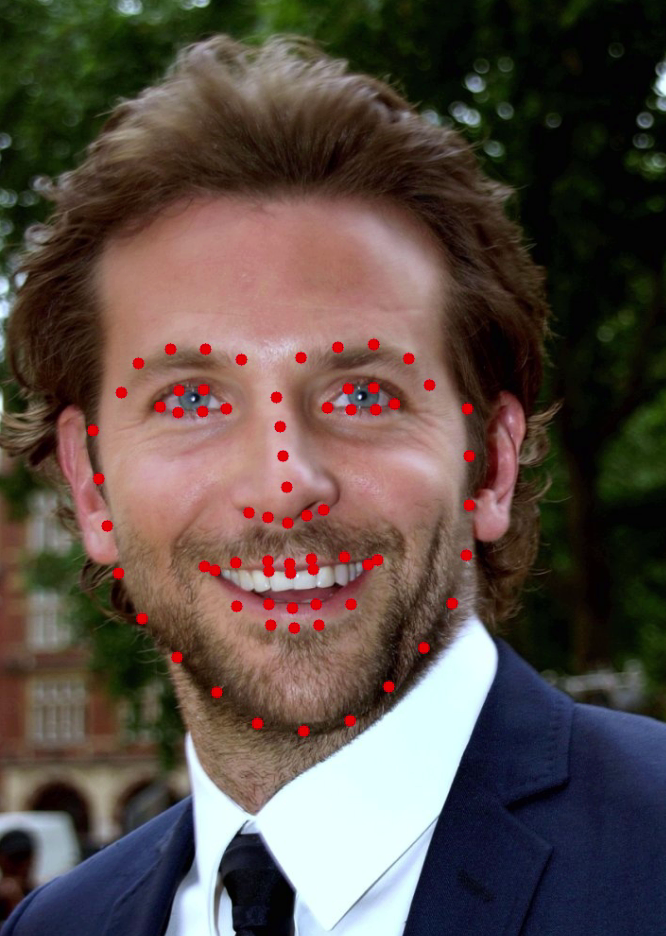
\includegraphics[scale=0.4]{figures/points.png}
        \caption{Placement des points caractéristiques du visage}
        \label{fig:Points}
	\end{minipage}\hfill
	\begin{minipage}[b]{0.48\linewidth}	
		\centering 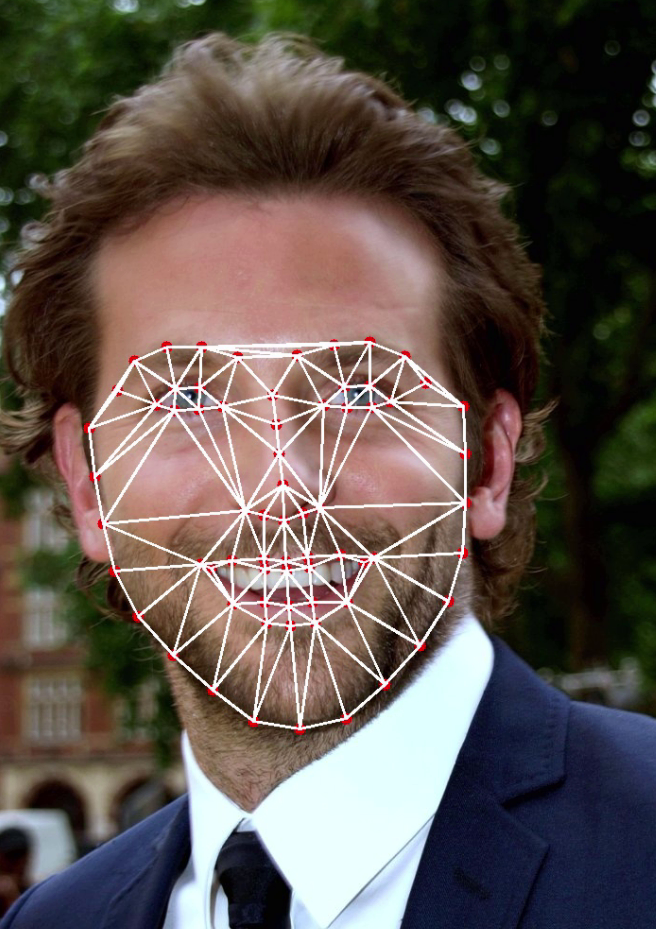
\includegraphics[scale=0.4]{figures/triangles.png}
        \caption{Placement des triangles selon les points caractéristiques}
        \label{fig:Triangle}
	\end{minipage}
\end{figure}

Selon le cahier des charges, l'échange de visages aurait dû recourir à nouveau à \textbf{OpenCV}. Mais le recours à un algorithme identifiant les points caractéristiques d'un visage n'a pu se faire avec \textbf{OpenCV}. C'est donc la bibliothèque \textbf{dlib}, massivement utilisée pour des transformations faciales, qui a été utilisée.\\ C'est grâce à la \textbf{classification linéaire SVM} (Support Vector Machine) de la bibliothèque \textbf{dlib} que le placement des points sur un visage est déterminé.\\

Le partitionnement du visage en triangles permet d'adapter le visage à copier selon l'expression du visage à remplacer comme l'illustre la déformation linéaire d'un triangle en figure \ref{fig:Lin_deforma}. Cela permet d'obtenir une meilleure cohérence quand à l'échange via une conservation des traits faciaux du visage de destination.\\
De ce fait, on peut observer le résultat d'une application de ce filtre en figures \ref{fig:Avant} et \ref{fig:Apres}. Cette façon d'échanger les visages possède cependant un défaut concernant certaines expressions antagonistes telles qu'un visage avec la bouche ouverte et le second avec la bouche fermée. Le programme essaye d'adapter la texture de la bouche fermée afin de simuler la personne souriante, ce qui n'est pas esthétique (il en est de même avec les yeux ou le port d'accessoires). Qui-plus-est, la difficulté des transformations n'a permis que l'échange de deux visages. Ce sont les deux visages les plus proches qui seront pris en considération pour cet échange.\\

\begin{figure}[H]
    \centering
    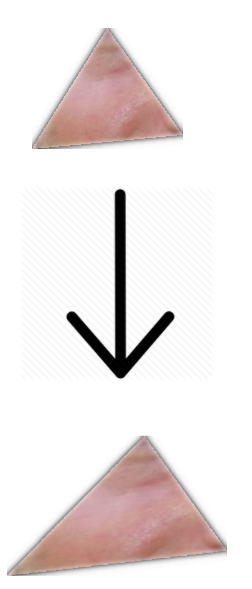
\includegraphics[scale=0.5]{figures/lin_deforma.png}
    \caption{Déformation linéaire d'un triangle}
    \label{fig:Lin_deforma}
\end{figure}
\begin{figure}[h!]
	\begin{minipage}[b]{0.40\linewidth}
		\centering 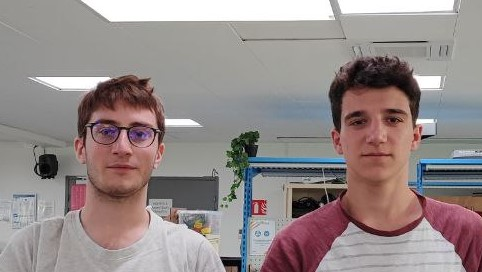
\includegraphics[scale=0.5]{figures/avant.jpg}
    \caption{Photo avant échange de visages}
    \label{fig:Avant}
	\end{minipage}\hfill
	\begin{minipage}[b]{0.48\linewidth}	
		\centering 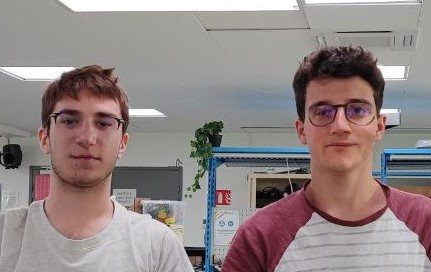
\includegraphics[scale=0.7]{figures/apres.jpg}
    \caption{Photo après échange de visages}
    \label{fig:Apres}
	\end{minipage}
\end{figure}

Une dernière fonctionnalité évoquée avec le client comme étant optionnelle consistait à donner un indicateur de similarité entre deux visages. Cependant le manque de temps a empêché le développement de cet objectif avancé cité dans le cahier des charges.\\

Ces deux filtres sont de plus utilisables aisément à tout endroit où une image est manipulée étant donné que les fonctions offrant ces services prennent une image en entrée et ressortent la même image modifiée. Cette modularité permet d'utiliser les filtres aisément dans le code source des machines à état, y compris pour appliquer une modification directement sur la capture vidéo (une proposition d'application avancée de filtres).

\subsubsection{Gestion des photos : Enregistrement, affichage et suppression}
Pendant des évènements de démonstration des capacités de Reachy, il nous sera utile de présenter aisément les photos récemment prises en les affichant de façon automatique sur un écran. Il faut également s'assurer de la sauvegarde des photos, étant une fonctionnalité requise par le client. De plus, les photos sont un point central parmi les données persistantes en mémoire que Reachy devra gérer. \'Etant donnée que Reachy est doté d'une mémoire finie, la gestion de l'accumulation des photos est un prérequis indispensable ayant besoin de définir une politique de suppression afin de déléguer cette gestion à un programme qui nous permettra, lors d'évènements, de nous focaliser sur les démonstrations du robot.\\

A chaque fois qu'une photo est prise, celle-ci est automatiquement enregistrée dans le dossier \textbf{tmp/img} servant de lieu de stockage des photos. Afin d'avoir un suivi temporel des photos, le nom des photos donné à l'enregistrement est sous la forme : \textbf{année\_mois\_jour\_heure\_minute\_seconde.png}\\
Cependant, cette information est à titre indicatif pour avoir un suivi visuel des moments où les photos sont prises. C'est grâce à la bibliothèque \textbf{os} que nous aurons connaissance des dates de création des photos afin d'apporter les traitements désirés.\\

Afin d'offrir un affichage des photos pendant les démonstrations de Reachy, un programme dédié est lancé en parallèle, en tant que processus indépendant de celui faisant fonctionner la machine à états. Celui-ci exploite la bibliothèque \textbf{os} afin de repérer quelle photo présente dans \textbf{tmp/img} est la plus récente et affiche en temps réel la photo trouvée sur un écran relié à Reachy par un câble HDMI grâce à une fonctionnalité de la bibliothèque \textbf{OpenCV}.\\
Cela permet aux utilisateurs de vérifier si leur photo est convenable afin de demander en directe à Reachy d'en prendre une nouvelle dans le cas non échéant. Cette fonctionnalité est exécutée en parallèle du programme de la machine à états afin d'avoir une meilleure maîtrise en temps réel de ce programme mais aussi par soucis de complexité du code quand à son insertion dans une machine à états.\\

De façon similaire au fonctionnement du programme précédent, la politique de suppression des photos est exécutée en temps réel par un processus fonctionnant en parallèle. La mémoire de Reachy étant limitée, nous nous sommes assuré de déléguer la tâche de suppression en temps réel d'un trop plein de photos à un programme. Celui-ci exploite également la bibliothèque \textbf{os} pour classer les photos présentes dans \textbf{tmp/img} par date de création et supprime les photos les plus anciennes.\\
Cette politique de suppression a été approuvée par le client. De plus, la fonction offrant ce service est paramétrable de telle façon que nous devons indiquer le nombre de photos maximum à partir duquel la suppression sera effectuée mais aussi le nombre de photos qui seront supprimées à chaque appel de cette fonction.\\
Ceci permet par exemple d'indiquer une limite de 500 photos et de demander la suppression de 50 photos en cas de dépassement de ce seuil. Ainsi, à 501 photos, la fonction en supprimera 50 et il en restera 451 de façon à ce que ce traitement ne soit appelé qu'après la création de 50 nouvelles photos (ce qui permet de temporiser l'appel à cette fonction).\\

Cette tâche pouvant être lourde selon le nombre de photos à traiter, nous avons prévu une attente passive de 10 secondes réveillant le processus via un signal grâce à l'utilisation de la fonction \textbf{sleep()} (temps jugé pertinent au vu de la faible fréquence de prise de photos de Reachy).\\
Il était spécifié dans le cahier des charges que lors d'un dépassement de la mémoire, un signal serait envoyé au administrateur afin de supprimer les photos par lancement manuel d'un programme et selon la même politique que le programme précédemment présenté. Cette autonomie, appréciée par le client, nous a permis de gagner en facilité de gestion de Reachy lors d'évènements.

\subsection{Détection des tags Arucos}
Les codes Aruco sont un pilier du fonctionnement de Reachy en cas de dysfonctionnement de la reconnaissance vocale et se sont révélés indispensables lors de la soirée partenaire. Ce sont des carrés similaires à des QR codes, avec un nombre de pixels généralement plus restreint et ayant pour objectif d'encoder un nombre entier naturel comme illustré en figure \ref{fig:Aruco}. Ces codes sont souvent utilisés pour identifier des objets facilement à partir d'un traitement d'image rapide.\\

\begin{figure}[H]
    \centering
    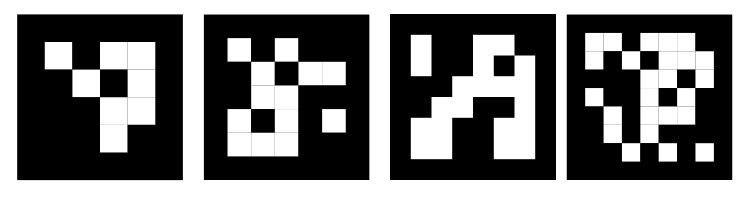
\includegraphics[scale=0.6]{figures/Aruco.png}
    \caption{Gamme de codes Aruco}
    \label{fig:Aruco}
\end{figure}

Pour notre projet nous avons décidé d'utiliser des Arucos de taille 4. Le fonctionnement de la détection et reconnaissance des codes Aruco est très similaire à celui des visages. Après identification de la surface plane définissant le code, la dimension de la matrice associée est déterminée et le calcul de la valeur représentée est effectué. Pour effectuer cela nous utilisons l'api \textbf{aruco} de \textbf{OpenCV}, celle-ci utilise un dictionnaire \textit{MARKER\_DIC} pour connaître l'ensemble des Arucos possible ainsi que la fonction permettant de detecter les Arucos \textit{PARAM\_MMARKERS}.\\
L'association entre des nombres et des transitions nous a permis de faire passer Reachy d'un état à un autre grâce à ses facultés visuelles. Cependant, le nombre de codes utilisés a impliqué une restriction des interactions orales possibles quant aux conversations.\\

\subsection{Mouvements}
En plus de la fonctionnalité d'assistance vocale et de prise de photo, le robot doit effectuer des mouvements pour le rendre plus attractif. Pour cela les mouvements qu'il effectue doivent être le plus naturels possible pour que ça se rapproche d'un comportement humain. Pour cela, le robot peut bouger sa tête à l'aide de trois moteurs combinés en un système appelé "orbita" ainsi que ses 2 antennes. Nous allons donc utiliser la combinaison des 2 pour effectuer les mouvements du robot. Comme dit dans le cahier des charges, nous avons utilisé l'API \textbf{reachy\_sdk} pour mouvoir Reachy.

\subsubsection{Faire différentes émotions}
Pour que Reachy ait certaines réactions humaines il nous fallait définir des positions pour que le robot donne l'impression qu'il ressent des émotions. Dans le cahier des charges nous avions défini 6 positions décrites dans les annexes.\\

La première modification qui a été apportée est de ne pas définir une position fixe pour chaque émotion, mais de définir des angles fixes à partir de la position initiale. Cela permettra au robot de faire l'émotion en face de l'utilisateur peut importe sa position. Nous avons donc décidé de décrire les mouvements du robot dans un repère sphérique. De plus, nous avons défini les attributs \textcolor{freeblue}{THETA} et \textcolor{freeblue}{PHI} qui stocke les angles auxquels se trouve l'utilisateur et \textcolor{freeblue}{TMP\_THETA} et \textcolor{freeblue}{TMP\_PHI} qui contiennent la position actuelle du robot. Avec THETA correspondant aux angles de rotation autour de l'axe y et PHI autour de l'axe z représentés sur la figure \ref{fig:repere}. THETA ayant la valeur de 0 quand il a la tête totalement vers le haut et PHI ayant la valeur de 0 quand il regarde en face de lui.

\begin{figure}[H]
    \centering
    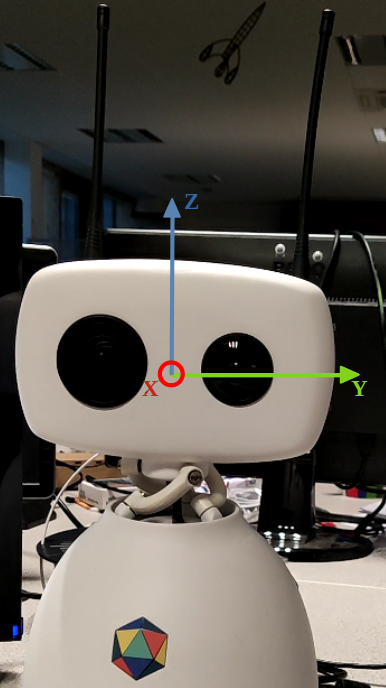
\includegraphics[scale = 0.25]{figures/repere.png}
    \caption{Repère pour les mouvements de la tête}
    \label{fig:repere}
\end{figure}

L'autre a été qu'au lieu de définir une durée que le robot doit mettre pour faire le mouvement, nous avons décidé de définir une vitesse. Cela permet à ce que peu importe la position d'où il se trouve et d'où il veut aller, il le fasse à la même vitesse. Cette modification permet de rendre le mouvement plus naturel. Avec uniquement une durée, il nous arrivait que le robot fasse un mouvement trop rapide et donc pas naturel, car il devait faire un petit mouvement pour aller de sa position initiale à sa position final ou au contraire un mouvement trop rapide pour faire un grand mouvement.\\

Les fonctions \textit{listen}, \textit{sad}, \textit{happy}, \textit{incentive}, \textit{thinking} et \textit{thanking} permettent respectivement à Reachy d'effectuer les émotions "écoute" \ref{ecoute}, "triste" \ref{triste}, "content" \ref{content}, "incitation" \ref{incitation}, "reflexion" \ref{reflexion} et "remerciement" \ref{remerciement} décrit dans le tableau ci-dessous \ref{tableau_position}.

\begin{center}
\label{tableau_position}
    \begin{tabular}{| c | c | c | c | c | c |}
        \hline
        Position & Angles tête & Vitesse tête & Angle antenne gauche & Angle antenne droite & Vitesse antennes \\
        \hline
        écoute & 0, 0 & 0.15 & 0 & 0 & / \\
        triste & 31.15, 0 & 0.13 & 140.0 & -140.0 & 70 \\
        content & 5.74, 0 & 0.15 & $\pm$20.0 & $\pm$20.0 & 300 \\
        incitation & -5.74, 0 & 0.1 & 35.0 & -35.0 & 70 \\
        réflexion & -16.13, 16.7 & 0.21 & -40.0 & 40.0 & 70 \\
        remerciement & 5.74, 0/26.51, 0 & 0.15/0.35 & -40.0 & 40.0 & 70 \\
        \hline
    \end{tabular}
\end{center}

\begin{figure}[!ht]
    \centering
    \begin{subfigure}{0.25\textwidth}
        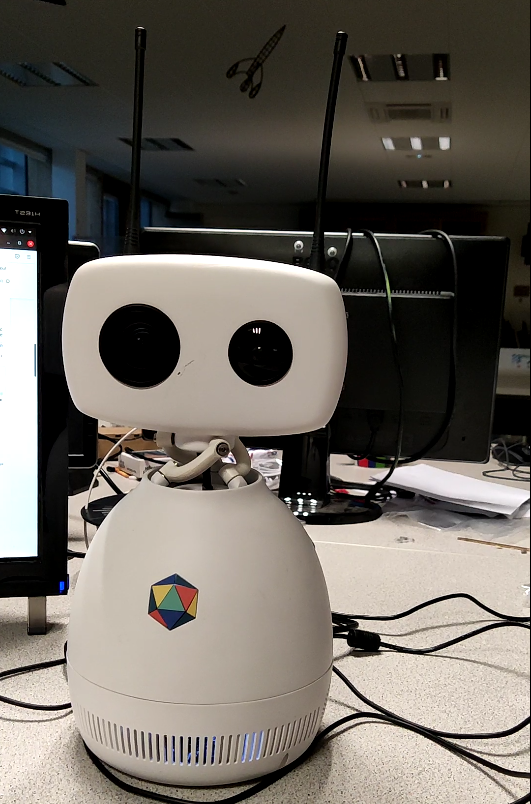
\includegraphics[width=\textwidth]{figures/ecoute.png}
        \caption{Emotion écoute}
        \label{ecoute}
    \end{subfigure}
    \begin{subfigure}{0.25\textwidth}
        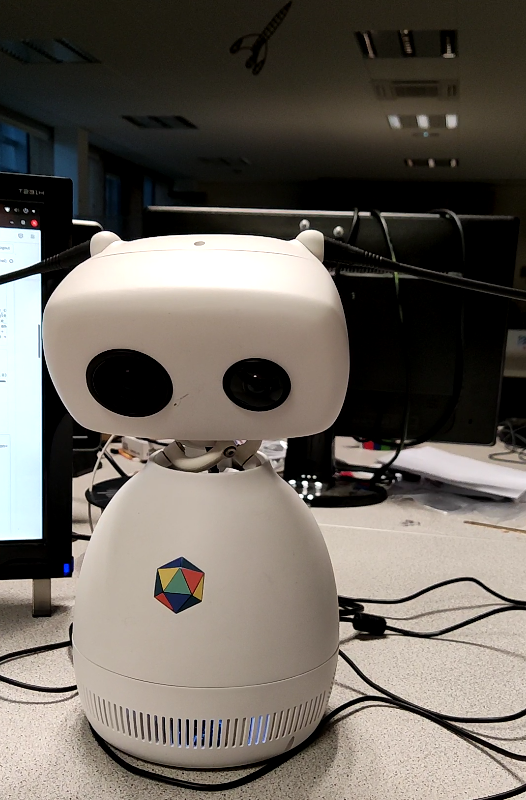
\includegraphics[width=\textwidth]{figures/triste.png}
        \caption{Emotion triste}
        \label{triste}
    \end{subfigure}
    \begin{subfigure}{0.25\textwidth}
        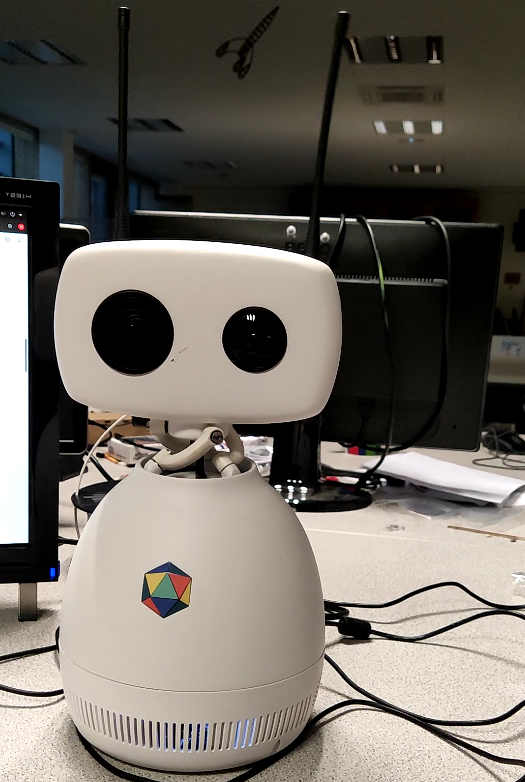
\includegraphics[width=\textwidth]{figures/content.png}
        \caption{Emotion content}
        \label{content}
    \end{subfigure}
    \begin{subfigure}{0.25\textwidth}
        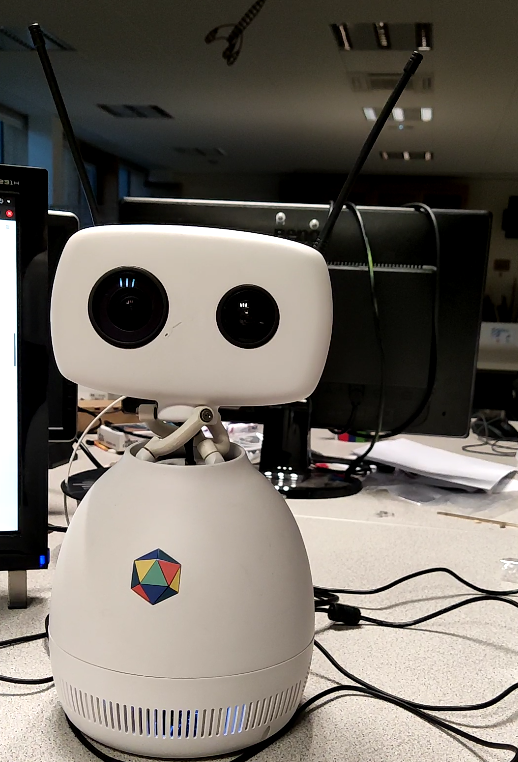
\includegraphics[width=\textwidth]{figures/incitation.png}
        \caption{Emotion incitation}
        \label{incitation}
    \end{subfigure}
    \begin{subfigure}{0.25\textwidth}
        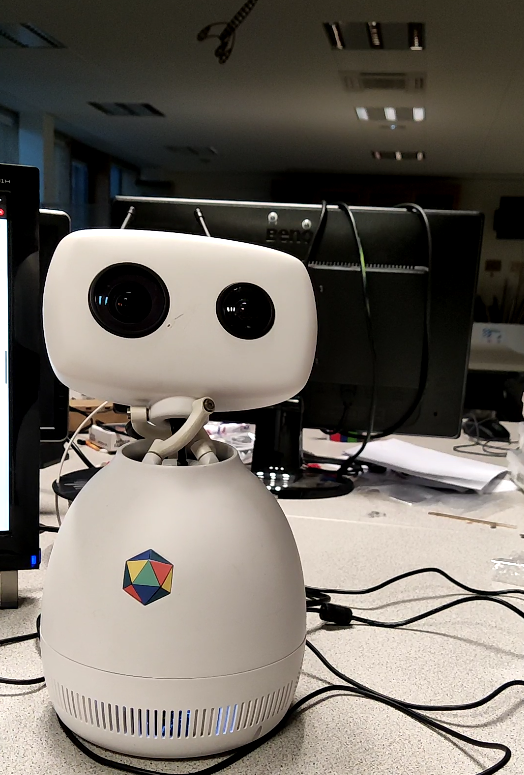
\includegraphics[width=\textwidth]{figures/reflexion.png}
        \caption{Emotion réflexion}
        \label{reflexion}
    \end{subfigure}
    \begin{subfigure}{0.25\textwidth}
        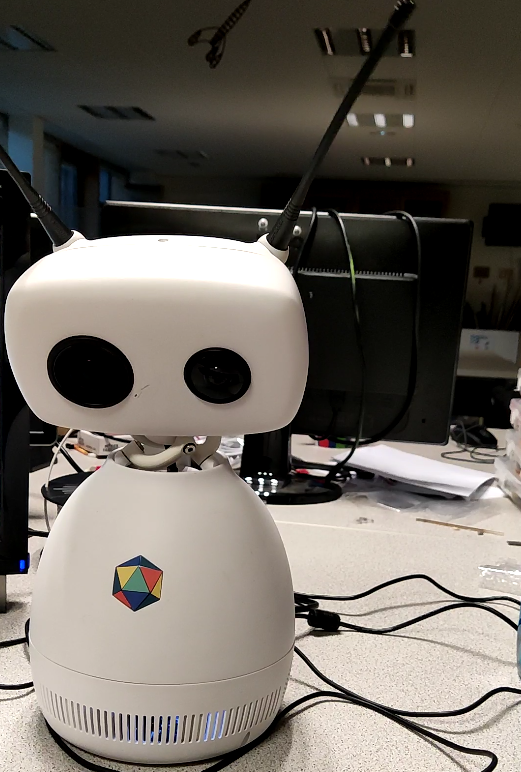
\includegraphics[width=\textwidth]{figures/remerciement.png}
        \caption{Emotion remerciement}
        \label{remerciement}
    \end{subfigure}
    \caption{Différentes émotions de Reachy}
\end{figure}

Une fois que le robot a fini de faire son émotion, il faut qu'il retourne à sa position initiale face à l'utilisateur. Cela signifie que les angles doivent repecter TMP\_THETA = THETA et TMP\_PHI = PHI, c'est la fonction \textit{move\_back} qui permet de le faire.\\

Comme défini dans le cahier des charges, nous avons mis en place 6 émotions différentes que nous considérions comme principales. Pour pouvoir avoir encore plus d'interaction avec l'utilisateur, il pourrait être intéressant d'en définir de nouvelles afin qu'il ait un comportement plus proche d'un humain.

\subsubsection{Suivi et cadrage des utilisateurs}
Une fois que les émotions ont été définies, il était fixé, dans le cahier des charges, que le robot suive le visage, de la personne avec qui il interagit, pour rendre le robot plus interactif. Pour cela, il nous a fallu relier la partie capture d'image avec la partie mouvement.\\

La mise en relation des 2 parties, nous a dans un premier temps posé quelques difficultés, car les directions des axes pour le mouvement et ceux de la capture d'image n'étaient pas les mêmes. Une fois la fonction de conversion déterminée, nous avons pu voir le robot déplacer sa tête à l'endroit où la personne se trouve. Dans un premier temps, pour effectuer ce mouvement nous avions utilisé la fonction \textit{look\_at} de l'api \textbf{reachy\_sdk} comme pour faire les émotions, mais cela générait un problème assez important. Ce problème était que lorsque le robot tournait la tête sur un axe horizontal, il penchait la tête sur le côté. Ceci était gênant pour l'aspect naturel du mouvement, mais surtout pour la capture d'image. Cette dernière ne pouvant pas prendre en compte le fait que le robot penche la tête sur le côté, faisant que le calcul des angles était biaisé et par conséquent le robot, n'ayant plus le bon angle, se décalait au cours du temps. Il était donc impossible d'avoir un bon fonctionnement du suivi des visages. \\

Nous avons fini par comprendre que pour regarder un point dans l'espace le robot a plusieurs possibilités de le faire. La fonction \textit{look\_at} ne permet pas de spécifier la manière dont nous voulons qu'il regarde. En regardant l'ensemble de l'api \textbf{reachy\_sdk}, nous avons remarqué que la fonction \textit{inverse\_kinematic} permet de choisir exactement la position de la tête du robot. La fonction \textit{inverse\_kinematic} prend en paramètres des quaternions pour pouvoir définir précisément la position des 3 moteurs déplaçant la tête de Reachy. Les quaternions sont des nombres complexes à 4 dimensions $Q\ =\ a+bi+cj+dk\ =\ [a\ b\ c\ d]\ =\ [cos(\frac{\Theta}{2})\ \ \ \ V_x*sin(\frac{\Theta}{2})\ \ \ \ V_y*sin(\frac{\Theta}{2})\ \ \ \ V_x*sin(\frac{\Theta}{2})]$ avec $V_x$, $V_y$ et $V_z$ les coordonnées du vecteur dans le repère cartésien et $\Theta$ l'angle de rotation autour de ce vecteur comme l'illustre la figure \ref{fig:quaternion}. Il était plus simple pour nous de décrire et visualiser les mouvements avec les angles d'Euler, nous avons donc implémenté la fonction \textit{\_\_euler\_to\_quaternion} permettant de faire la conversion des angles d'Euler en quaternions. Une fois les valeurs du quaternions souhaités obtenus, nous déplaçons la tête dans la position voulue à l'aide de la fonction \textit{update\_position}. Le passage par la cinématique inverse nous a permis de résoudre le problème que nous avions rencontré. \\ 

\begin{figure}[!ht]
    \centering
    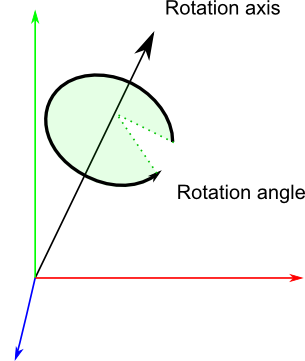
\includegraphics[scale = 0.5 ]{figures/quaternion.png}
    \caption{Représentation quaternions}
    \label{fig:quaternion}
\end{figure}

Reachy arrive donc bien à suivre le visage de l'utilisateur. Il lui manque cependant un peu de réactivité dans le suivi, mais cela reste tout de même acceptable.\\

Pour la prise de photo et surtout le cadrage de la photo, il est nécessaire que Reachy tourne sa tête vers la personne (ou le groupe de personnes) qui souhaite être prise en photo. Ayant déjà réussi le suivi de visage, le cadrage de la photo peut être considéré, du point de vue du mouvement, comme une partie de celui-là. C'est-à-dire qu'à partir des angles, permettant le cadrage, l'appel à la fonction \textit{update\_position} va orienter la tête de Reachy dans la bonne position pour prendre la photo comme s'il ne suivait qu'une unique fois un visage.

La partie cadrage ne nécessitant qu'un seul mouvement, il n'y a pas de problème de fluidité.

\subsubsection{Ressemblance aux mouvements humain}
Un point important du cahier des charges était que les mouvements devaient être les plus naturels possible. Donc une fois que nous sommes arrivés à ce que Reachy fasse les mouvements vers la direction que l'on souhaitait, il nous a fallu réfléchir ce qui faisait que son mouvement ne semblait pas naturel pour un être humain. Plusieurs aspects nous ont semblé importants de corriger pour qu'il se rapproche plus d'un comportement humain.\\

Tout d'abord contrairement à un humain qui est limité dans ces mouvements à cause de ces différentes articulations, le robot lui n'a pas de contrainte physique qui le limite dans ses mouvements. Donc dans un premier temps pour ne pas endommager le câble qui est situé à l'arrière de sa tête, permettant la communication entre ses différents capteurs et son unité de traitement, nous ne lui demandions pas de tourner sa tête à plus de 180 degrés sur l'axe horizontal. Cela était tout de même risqué car rien, de manière physique ou logiciel, ne lui empêchait de faire un mauvais mouvement. De plus, pour qu'il se rapproche plus d'un comportement humain, il ne fallait pas simplement l'empêcher de faire un angle plus grand que 180 degrés, mais le limiter à l'angle maximal qu'un humain peut faire, que ce soit sur l'axe vertical ou horizontal. Nous avons donc regardé les angles maximums moyens qu'un être humain peut faire dans les différentes positions. Nous sommes arrivés aux valeurs suivantes :
\begin{itemize}
    \item[-] axe vertical vers le haut : 45 degrés
    \item[-] axe vertical vers le bas : 40 degrés
    \item[-] axe horizontal vers la gauche : 45 degrés
    \item[-] axe horizontal vers la droite : 45 degrés
\end{itemize}
Une fois que nous avions déterminé ces valeurs, nous avons implémenté la fonction \textit{\_\_fit\_angles} permettant de manière logicielle de limiter le mouvement de la tête du robot. Cette fonction est appelée à chaque fois avant de demander au robot de bouger. Elle va dans un premier temps regarder si l'angle duquel nous souhaitons bouger est bien dans l'intervalle, si c'est le cas, il ne fait rien sinon il modifie la valeur de l'angle duquel le robot va se déplacer vers la limite la plus proche. Cela signifie que si on demande de tourner la tête de 60 degrés vers la droite et de 46 degrés vers le haut, il tournera finalement de 45 degrés vers la droite et le 45 degrés vers le haut.\\

Ensuite, nous avons rencontré un problème par rapport à la vitesse de mouvement de la tête. Au début, nous avions défini une durée du mouvement peu importe la rotation qu'il devait effectuer. Cela faisait que pour certains mouvements il allait très doucement et que pour d'autres au contraire, il allait très vite. Cela n'est pas très naturel, car en principe un être humain se déplace à la même vitesse peu importe le mouvement qu'il effectue. Nous avons donc décidé de définir pour chaque mouvement et émotions une vitesse fixe. Les fonctions \textit{look\_at} et \textit{goto} de l'api \textbf{reachy\_sdk} prennent en paramètre la durée du mouvement et non pas la vitesse. Nous avons donc créé la fonction \textit{\_\_duration} qui calcule la durée que le mouvement va mettre en fonction de la vitesse souhaitée, de la position où il se trouve et de la position vers laquelle il se dirige. \\

Finalement, une fois les problèmes précédents résolus, pour rendre le mouvement encore plus naturel, nous avons essayé de fluidifier le mouvement. Nous avons évité d'enchaîner trop rapidement de petits mouvements pour que la tête de Reachy ne fasse pas des à-coups. Les mouvements que fait le robot sont donc fluides, mais il serait possible encore de les améliorer. C'est surtout le cas pour la partie suivi de visage qui en calculant le prochain endroit à atteindre avant d'avoir fini le mouvement en cours pourrait être moins saccadé. Cela permettrait d'éviter qu'il s'arrête pour repartir ainsi que de rendre le suivi plus précis. Cependant avec les fonctions utilisées de l'api \textbf{reachy-sdk}, il est obligatoire de finir le mouvement avant d'en faire un autre à la suite. Une amélioration qui serait possible serait d'utiliser une interpolation différente de celle linéaire pour que le mouvement soit légèrement plus naturel.

\section{Mise en place et utilisation du robot / Manuel d'utilisation}

Cette partie vise à expliquer comment faire fonctionner le robot sur les machines à états déjà implémentées du branchement du robot jusqu'à l'exécution de la \texttt{State\_Machine}. Elle décrit également comment créer une nouvelle machine à états et l'exécuter. 

\subsection{Mise en place et matériel nécessaire}
Le Reachy Mini est en fait un ordinateur sous Linux, de ce fait, la mise en place se fait comme celle d'un PC. Il est pourvu de 2 ports USB  (voir \texttt{\color{red}{(2)}} sur la Figure \ref{fig:connectique}), 2 ports HDMI  (voir \texttt{\color{red}{(3)}} sur la Figure \ref{fig:connectique}) et un port d'alimentation (voir \texttt{\color{red}{(1)}} sur la Figure \ref{fig:connectique}). Il est donc nécessaire d'avoir un clavier et une souris pour les brancher aux 2 ports USB afin de naviguer dans le Reachy comme avec un PC. Le microphone ne fonctionnant pas très bien, il y a la possibilité de brancher un microphone externe via un casque-micro ou bien un micro seul. Pour cela il faut se munir d'un hub USB et le brancher à l'un des 2 ports USB puis y brancher le clavier, la souris et le micro. Ensuite pour ce qui est du visuel il faut brancher un écran sur l'un des ports HDMI. Durant le projet nous n'avions que des écrans avec entrée VGA, c'est pourquoi nous avons utilisé un adaptateur HDMI vers VGA, il est donc possible d'utiliser un adaptateur en fonction des besoins si vous ne disposez pas d'un écran avec entrée HDMI. Enfin, il suffit de brancher le câble d'alimentation du Reachy et de l'écran et la partie connectique est prête.

\begin{figure}[H]
    \centering
    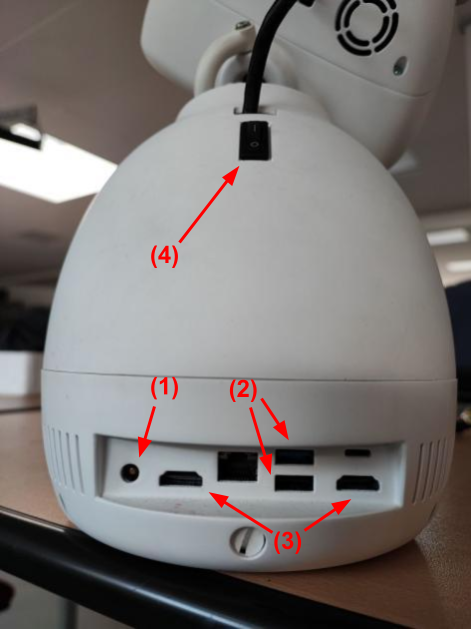
\includegraphics[scale=0.4]{figures/connectique.png}
    \caption{Différentes connectiques du Reachy et bouton d'activation des moteurs}
    \label{fig:connectique}
\end{figure}
  
Maintenant que le Reachy est branché, il suffit d'appuyer sur le bouton d'allumage de celui-ci qui est placé sur son torse (voir sur la Figure \ref{fig:allumage}). Ensuite l'ordinateur s'allume et nous pouvons naviguer comme sur tout autre ordinateur Linux via l'écran, le clavier et la souris.
 
\begin{figure}[H]
    \centering
    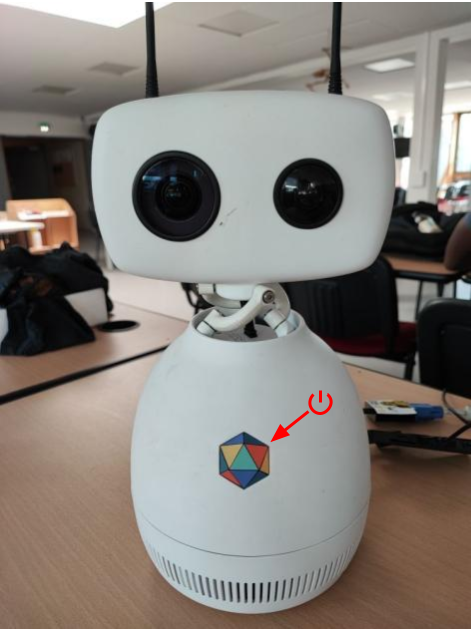
\includegraphics[scale=0.35]{figures/allumage_reachy.png}
    \caption{Position du bouton d'allumage du Reachy}
    \label{fig:allumage}
\end{figure}
  
\subsection{Initialisation du robot}
Tout d'abord il faut se placer dans le dossier du projet dont le chemin est \texttt{home/gitdir/PFA-Reachy-mini}, par la suite, toutes les commandes sont à effectuer depuis la racine du projet. \\
Avant de lancer une machine à états, il faut installer toutes les librairies et modules nécessaires à son utilisation. Pour cela, il faut exécuter la commande :
\begin{center}
\texttt{\$ make install}
\end{center}

Également, il est nécessaire de rafraîchir les serveurs du robot avec la commande :
\begin{center}
\texttt{\$ make reload-server}
\end{center}

En effet, cela permet d'éviter quelques soucis de connexion. \\

Ensuite, il est nécessaire d'effectuer le focus de la caméra du Reachy. Pour cela il faut tout d'abord activer les moteurs du robot en appuyant sur l'interrupteur placé sur le dos du robot (cf \texttt{\color{red}{(4)}} Figure \ref{fig:connectique}). Ensuite, il faut lancer le programme \texttt{Python} dédié au focus. Celui-ci peut être exécuté via la commande :
\begin{center}
\texttt{\$ make initiate-camera}
\end{center}

Une fenêtre va s'afficher avec le retour vidéo du Reachy. Il vous faudra alors placer votre main proche de la caméra pour que le Reachy fasse le focus sur elle (cf Figure \ref{subfig:etape1}). Puis l'éloigner petit à petit en lui laissant le temps de faire les focus successifs (cf Figures \ref{subfig:etape2}). Enfin, lorsque l'image semble nette (cf Figure \ref{subfig:etape3}) il faut appuyer sur la touche \texttt{Q} de votre clavier pour fixer le focus. Il est tout à fait possible de refaire le focus s'il ne vous convient pas en refaisant la même manipulation. \\

\begin{figure}[!ht]
    \centering
    \begin{subfigure}{0.25\textwidth}
        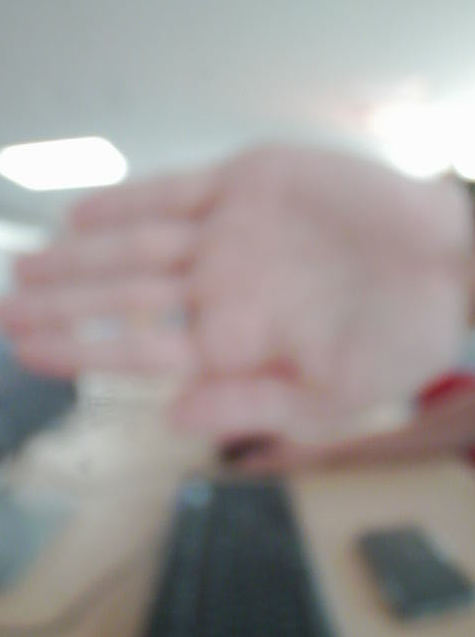
\includegraphics[width=\textwidth]{figures/etape1.png}
        \caption{Etape 1}
        \label{subfig:etape1}
    \end{subfigure}
    \begin{subfigure}{0.25\textwidth}
        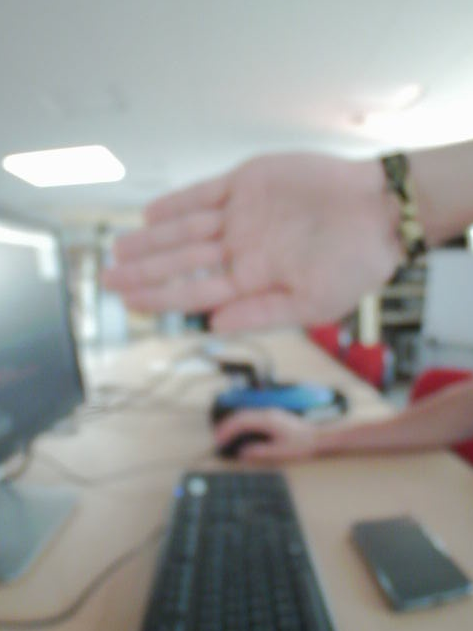
\includegraphics[width=\textwidth]{figures/etape2.png}
        \caption{Etape 2}
        \label{subfig:etape2}
    \end{subfigure}
    \begin{subfigure}{0.25\textwidth}
        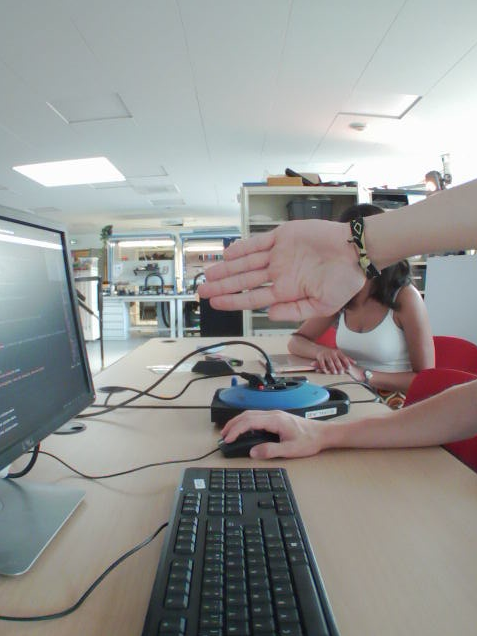
\includegraphics[width=\textwidth]{figures/etape3.png}
        \caption{Etape 3}
        \label{subfig:etape3}
    \end{subfigure}
    \caption{Suite d'images expliquant les étapes d'initialisation de la caméra du Reachy}
\end{figure}

Cela termine la partie mise en place du robot.

\subsection{Utilisation du robot} \label{subsec:utilisation}
Afin de décider des fonctionnalités du robot, il faut se servir de la partie sur la machine à états (cf \ref{section_machine_etat}. Il faut donc tout d'abord créer un fichier \texttt{.json} comme l'annexe \ref{subsec:annexe_json} en spécifiant les états, les transitions, les actions et prédicats associés et en le plaçant dans le dossier \texttt{/PFA-Reachy-mini/assets/json}. Ensuite, il faut créer un fichier considéré comme \texttt{module} de la machine à états c'est-à-dire un fichier avec l'implémentation de l'ensemble des fonctions demandées par la \texttt{State\_Machine}. Celui-ci devra être placé dans le dossier \\ \texttt{PFA-Reachy-mini/src/state\_machine}. Avec le fichier \texttt{.json} et le fichier \texttt{module}, il est ensuite possible de lancer le Reachy sur cette machine à états. Pour cela il faut rajouter une règle dans le \texttt{Makefile} en copiant par exemple la règle \texttt{reachy-final} et en remplaçant son nom par le nom voulu, la description de la machine par la description souhaitée et le fichier \texttt{state\_machine\_final.json} par le nom de notre fichier \texttt{.json}.\\

Cette partie présente comment lancer une machine à états quelconque et présente celle déjà présente dans le robot et comment faire exécuter par Reachy.

\subsubsection{Machine à états quelconque}
Pour exécuter une \texttt{State\_Machine} sans passer par le \texttt{Makefile} il faut se rendre dans le dossier \\ \texttt{/PFA-Reachy-mini/src/state\_machine}. Ensuite il faut lancer un programme \texttt{Python} en lui spécifiant le chemin relatif vers le fichier \texttt{.json} de la machine. Pour cela il suffit d'exécuter la commande suivante :
\begin{center}
\texttt{python3 reachy\_state\_machine\_argv.py \textit{<chemin relatif vers le .json>}}. \\
\end{center}

Ceci est la méthode pour lancer n'importe quelle machine à états à partir de son fichier \texttt{.json}. Nous allons maintenant donner les méthodes pour lancer les 2 machines principales du projet.

\subsubsection{Machine à états "Only Aruco"}
La première est la machine à états qui n'utilise que les codes Aruco. Il faut donc se munir des 16 premiers codes Aruco afin de pouvoir utiliser toutes ses fonctionnalités. Il est possible d'avoir une conversation basique avec le robot, de prendre une photo de groupe, une photo simple, d'effectuer un échange de visage et une photo en noir et blanc. Pour exécuter cette machine à états et donc cette version du robot, la commande à utiliser est : 
\begin{center}
    \texttt{make reachy-only-aruco}.
\end{center}

\subsubsection{Machine à états "finale"}
Il s'agit de la machine à états la plus aboutie. Le robot attend tout d'abord d'entendre "Hey Reachy" avant de s'activer. Puis écoute la personne. Il est capable de reconnaître différents mots-clés et dans le cas où il ne reconnaît rien il fait appel à l'IA \texttt{GPT-3}. Il est également capable des mêmes capacités en termes de prise de photo que le "Only Aruco". Pour exécuter cette machine à états et donc cette version du robot, la commande à utiliser est : 
\begin{center}
    \texttt{make reachy-final}.
\end{center}


\subsection{Autres programmes utiles}

Cette partie décrit les programmes annexes pouvant être exécutés en parallèle du Reachy afin d'effectuer la gestion des images prises par le robot.

\subsubsection{Programme d'affichage des photos}
Lors de la prise de photos, celles-ci sont stockées dans le Reachy. Il est possible de les afficher en temps réel en lançant le programme dédié en parallèle de la \texttt{State\_Machine}. Pour cela il suffit de lancer la commande suivante : 
\begin{center}
    \texttt{\$ make show-last-img}
\end{center}

Cela va afficher une fenêtre avec la dernière photo prise, cela ne s'actualise pas automatiquement si le Reachy prend une photo, il faut presser la barre espace afin de rafraîchir la fenêtre. Ce programme a été développé pour permettre l'affichage des photos en plein écran, ainsi il est préférable d'utiliser un deuxième écran afin de pouvoir afficher les images et manipuler le robot en même temps. Cependant, il est tout à fait possible d'utiliser \texttt{ALT + TAB} pour basculer entre les deux.

\subsubsection{Programme de suppression de photos}
La mémoire du Reachy est bien entendu limitée, c'est pourquoi nous avons mis en place un programme de suppression de photos. Celui-ci peut se lancer en parallèle d'une machine à états et de l'affichage des photos. Son rôle est de supprimer les photos les plus anciennes si le Reachy a déjà enregistré \texttt{N} photos. Le programme permet donc la suppression de \texttt{P} photos à partir du moment où il y a \texttt{N} photos ou plus dans le répertoire de stockage des photos. \texttt{N} et \texttt{P} sont donc les arguments à donner en ligne de commande. Ainsi, pour le lancer il faut exécuter la commande suivante :
\begin{center}
    \texttt{\$ make delete-images NB\_PHOTOS=\textit{<N>} NB\_TO\_DELETE=\textit{<P>}}
\end{center}

Par défaut, le nombre d'images à stocker avant suppression est fixé à 100. Et dès que cette valeur est atteinte, 2 images sont supprimées.


\section{Les limites du robot et les améliorations possibles du projet}
Lors de ce projet, nous avons manipulé Reachy sous différents aspects. Ainsi, certains aspects positifs et négatifs ont été repérés et cette partie va permettre de lister ces caractéristique afin d'offrir à Pollen Robotics des voies d'amélioration possible du robot Reachy Mini, et également afin d'expliquer pourquoi certaines parties du projet ont été plus ou moins efficaces.

\subsection{Les qualités et défauts de Reachy Mini}
\textbf{Qualités}\\\\
Tout d'abord, le robot présente de nombreux avantages qui facilitent sa manipulation. La grande modularité de ses fonctions était un atout très important pour permettre une avancée rapide de notre projet. \\
En effet, comme nous manipulions différentes parties du robot, il était très utile que la synthèse vocale, les mouvements et les caméras du robot soient manipulables de façon modulaire. \\

\'Egalement, la présence de nombreuses fonctions bas niveau est un grand atout. Par exemple, pour les mouvements, le fait de pouvoir contrôler la tête du robot avec les méthodes \texttt{look\_at} et \texttt{goto} permet de contrôler sa tête de deux façons, la première concernant le regard du robot, et la deuxième utilisant directement les angles des joints liants la tête au corps. Ainsi, la mise en place des émotions, et des mouvements et leur différenciation a été facilitée par l'utilisation de ces méthodes. \\

\textbf{Défauts}\\\\
Cependant, le robot présente tout de même quelques défauts. Le premier défaut que nous avons constaté concerne les mouvements. Il semblerait que le robot garde en mémoire (en cache) le mouvement qu'il est en train de réaliser. Nous avons eu plusieurs fois des segmentation fault lors de ce projet et si nous rallumions le robot, alors la première chose qu'il cherchait à faire lors de l'appel à une fonction de mouvement, était de faire le dernier mouvement qu'il avait essayé de faire et qui n'était pas encore terminé. Ainsi, nous avons plusieurs soucis liés à cela, sans réellement trouver la cause de ce redémarrage. Cependant, après avoir mis des vérifications sur les angles envoyés aux fonctions de mouvement, nous n'avons plus eu ce problème, car le robot ne faisait que des mouvements "valides" et donc ne crashait plus de cette façon. \\

Un autre défaut, plus important cette fois-ci, concerne le micro du robot. Nous avions besoin de ce micro pour la reconnaissance vocale. Cependant, bien qu'il capte parfaitement la direction du son (micro multi-directionnel), il n'était pas en mesure de capter suffisamment le son pour que le robot comprenne ce qui était dit. Même une fois la réduction de bruit mise en place, le robot captait le son, dans la bonne direction, mais il ne captait pas les paroles réellement prononcées. \\
Nous avons essayé ce micro de façon externe au robot avec une carte audio supplémentaire. Cependant, nous avons obtenu les mêmes problèmes. Enfin, en ajoutant un micro externe au robot, tel qu'un casque-micro, alors le son est parfaitement capté. Le soucis provient donc bien du micro utilisé dans le robot. \\ Ainsi, il a été impossible d'utiliser le micro directionnel permettant au robot de s'orienter vers le son. \\

Enfin, un autre défaut du robot a été l'utilisation de ses caméras. Il se trouve que le focus était compliqué à réaliser car les caméras fixaient automatiquement les micro-poussières présentes à l'intérieur de la lentille. Pour contrer cela, nous avons choisi de réaliser le focus une unique fois à l'initialisation du robot, puis de ne plus y toucher. On pouvait ainsi avoir un réel aperçu du focus et le calibrer comme nous le souhaitions. De plus, une fois le focus calibré, il permet la netteté d'une grande zone du champ de vision du robot, il n'est donc pas nécessaire de le refaire à chaque fois.

\subsection{Améliorations possibles de notre projet}
\textbf{Envoi des photos} \\ 

En ce moment, toutes les photos prises par Reachy sont sauvegardées localement. Une façon plus sophistiquée de le faire serait de faire une interface qui affiche un champs de texte pour que chaque utilisateur puisse rentrer son adresse e-mail, et par la suite on pourra la lui envoyer. \\

\textbf{Utilisation des deux caméras} \\

Pour des soucis de simplification, nous avons fait le choix de n'utiliser que la caméra droite du robot. En effet, elle procure un angle suffisamment grand pour être utilisée toute seule. Une amélioration possible du projet serait d'utiliser les deux caméras et de les exploiter de telle sorte qu'elles ne forment qu'une seule caméra plus performante.\\

\textbf{Ajouts d'émotions} \\ 

Les émotions que Reachy peut exprimer jusqu'à présent sont limitées à six émotions : \texttt{écoute}, \texttt{triste}, \texttt{content}, \texttt{incitation}, \texttt{réflexion}, \texttt{remerciement}. Ces émotions ne peuvent pas être exprimées au milieu d'une conversation avancée. Alors deux améliorations sont envisagées dans ce cas : d'abord, nous souhaitons ajouter plus d'émotions comme par exemple \texttt{ennuyé} ou \texttt{surpris}, et nous voulons intégrer un algorithme d'apprentissage automatique qui analyse, au fur et à mesure, toutes les phrases de l'utilisateur, et ce au milieu de la conversation avancée, et qui donne trois réponses : \texttt{positif}, \texttt{négative} ou \texttt{neutre}. Par la suite, nous associons le mouvement associé à chacune de ces réponses. Ceci peut être également fait avec l'API \textbf{OpenAI}.\\

\textbf{Parallélisation des fonctions de détection} \\ 

Actuellement, nous avons deux machines à états différentes pour interagir avec le robot soit avec des codes Aruco, soit avec la voix. Une amélioration sur laquelle nous avons commencé à travailler est la parallélisation des processus. En effet, il serait très utile que le robot puisse, tout en écoutant ce qu'il se passe autour de lui, observer les choses et donc détecter des codes aruco. De même, cela permettrait de réaliser de nombreuses actions en parallèles sans forcément utiliser les fonctions asynchrones de l'API \texttt{reachy-sdk}. \\ Nous avons commencé à implémenter cette amélioration, cependant nous avons rencontré des soucis avec \texttt{PyAudio} qui n'aimait pas être exécuté en parallèle à un autre programme. \\ Nous avons donc choisi de nous concentrer sur les autres fonctionnalités quitte à faire deux machines à états différentes plutôt que s'obstiner à faire marcher une unique machine à états qui n'aurait pas eu toutes les fonctionnalités. \\

\textbf{Utilisation du micro directionnel en plus d'un autre micro} \\ 

Une amélioration possible serait de combiner la fonctionnalité du  micro associé au robot qui détecte la direction du son avec l'autre micro que nous avons ajouté qui détecte bien le son et les paroles afin d'avoir un bon rendement au niveau de la détection du son.

\section{Évènements de présentation du projet}
L'un des objectifs finaux du projet était de pouvoir présenter Reachy lors de différents événements. Cela permettant aux différents participants de pouvoir se prendre en photo sur demande.

\subsection{Soirée Partenaires}
Le premier événement auquel il a vraiment participé a donc été la soirée partenaire de l'ENSEIRB-MATMECA. Cela nous a permis de présenter notre travail à certains des élèves ainsi qu'aux partenaires de l'école.\\

En prenant en compte le niveau sonore du bruit dans la pièce de l'événement, nous avons préféré ne pas utiliser la partie reconnaissance vocale du robot. Pour cela nous avons donc mis en place une machine à états où la communication des ordres ne s'effectue qu'à l'aide des tags aruco.\\

Même si la commande vocale ne fonctionnait pas, les tags arucos ont permis d'effectuer la plupart des fonctionnalités du robot. Reachy effectuait les mouvements et émotions correspondants aux actions et aux commandes demandées. Par exemple lorsque nous lui montrions le tag correspondant à "tu est mignon", le robot faisait l'émotion "content". Reachy pouvait aussi tourner la tête pour détecter et suivre la personne face à lui. L'utilisateur pouvait ainsi lui demander de prendre une photo, seul ou en groupe. Reachy cadrait donc la photo en bougeant la tête avant de prendre la photo et de l'afficher sur l'écran. L'utilisateur pouvait aussi demander au robot de lui raconter une histoire. A l'aide d'\textbf{openIA} et du contexte de l'événement donné en paramètre, Reachy pouvait donc raconter des histoires en relation avec la soirée partenaire.\\

Cet événement a donc été très intéressant pour montrer les différentes fonctionnalités du robot que nous avons implémentées ainsi que de prendre en compte les remarques des utilisateurs afin de l'améliorer davantage.

\subsection{100 ans de l'ENSEIRB}
Les 100 ans de l'ENSEIRB était l'événement majeur cité dans le cahier des charges. Le robot devait être fonctionnel et être présenté pour cet événement. Cependant, à cause des circonstances actuelles, les 100 ans de l'ENSEIRB n'ont pas eu lieu à la date initiale. Il est cependant prévu que cet événement soit reporté à début septembre de cette année. Si cela est possible, nous essayerons d'y participer afin de montrer le fonctionnement et l'ensemble des possibilités que Reachy offre en espérant que cette fois-ci nous pourrons utiliser la partie reconnaissance vocale malgré le monde et le bruit qu'il y aura. 

\newpage
\section{Conclusion}
Le Projet au Fil de l'Année a été un projet intense dont le management n'a pas été très facile à gérer dû au grand nombre de personnes dans le groupe. Ainsi, des rôles se sont naturellement formés au sein du groupe pour assurer une bonne coopération. Par exemple, Lucas gérait la communication avec le client et l'encadrant, Clara mettait en commun les différents modules du code, et chacun des autres membres était concentré sur l'élaboration de sa partie et de sa bonne réalisation. \\

De plus, nous n'avions pas de créneaux réservés à la réalisation du projet dans nos emplois du temps respectifs. Mais nous avions la contrainte de travailler avec le robot pour certaines parties comme celle des mouvements. Ainsi, il a fallu trouver des créneaux communs pour travailler. En général, nous nous retrouvions le jeudi matin, et en début d'après-midi pour travailler sur le robot (les parties non faisables à la maison notamment) puis nous enchaînions par une réunion avec l'encadrant ou le client. \\

M. \textsc{Rollet} était notre encadrant, bien que M. \textsc{Morandant} ait également participé à la gestion du projet. Ce regard nouveau sur la réalisation, nous a permis d'obtenir un nouvel avis, et a été un moteur pour la suite du développement du projet. En effet, les bases ayant été fixées par M. \textsc{Rollet} et le groupe de PFA et le développement de ces-dernières ayant déjà été commencé, M. \textsc{Morandat} a pu avoir un regard extérieur et soulever des contraintes et améliorations auxquelles nous n'avions pas encore réfléchis. Ce qui constituait ainsi une petite perte de temps car il fallait revoir quelques parties de l'implémentation, a finalement permis de gagner en rapidité sur la suite du projet (par exemple avec la nouvelle façon de créer des machines à états à l'aide des json). \\

Lors de l'intégralité du projet, nous pouvions entrer en contact avec des membres de Pollen Robotics. En effet, nous avions été ajoutés au serveur Discord de l'entreprise par M. \textsc{N'Guyen}. Cela nous a permis notamment d'obtenir des informations supplémentaires sur certaines documentations que nous ne trouvions pas sur le Github de Pollen Robotics. Cette aide a donc été précieuse afin de poser nos questions directement aux personnes connaissant le robot et ses fonctionnalités. \\

Ainsi, le PFA sur le robot Reachy a été un projet innovant pour l'ensemble du groupe. Nous avons apprécié travailler sur différents aspects (mouvement, caméra, audio, ...) et sur un projet concret. Voir concrètement le robot bouger ou parler à la suite de l'implémentation de certaines fonctions était très motivant pour la suite du projet. \\

\textbf{Remerciements} \\

L'ensemble du groupe tient à remercier M. \textsc{Rollet} Antoine, encadrant du projet, ayant suivi le groupe tout au long du projet, même à distance.\\

Nos remerciements vont également à M. \textsc{Morandat} Floréal, qui a permis la continuité pédagogique lors du remplacement temporaire de M. \textsc{Rollet}. Son regard extérieur a permis de faire émerger de nouvelles idées qui ont favorisé la réalisation du projet. \\

Merci à M. \textsc{Janin} David pour la gestion des PFA, la proposition des sujets et les informations diverses qu'il a pu partager. \\

Nous tenons également à remercier M. \textsc{N'Guyen} Steve pour avoir proposé ce projet en tant que PFA, et nous avoir fait confiance dans la réalisation de ce dernier. Son aide a également été précieuse pour comprendre le robot et son API. \\

Nous remercions aussi \textsc{Pollen Robotics} et l'ensemble de ses membres pour leur réactivité sur le serveur Discord, mais également pour le prêt du robot sans qui le projet n'aurait pas eu lieu.

\newpage
\section*{Bibliographie}
\textbf{Figure \ref{fig:quaternion}} : image représentation des quaternions\\
\url{http://www.opengl-tutorial.org/fr/intermediate-tutorials/tutorial-17-quaternions/}
\\

\textbf{Figure \ref{fig:Points}, \ref{fig:Triangle} et \ref{fig:Lin_deforma}} : face swapping \\
\url{https://pysource.com/2019/05/28/face-swapping-explained-in-8-steps-opencv-with-python/}



\label{RealLastPage}
\newpage
\thispagestyle{fancy}
\fancyfoot[R]{}
\section{Annexes}
\subsection{Cahier des charges}
%\import{./Cahier_des_charges}{cahier_des_charges.tex}
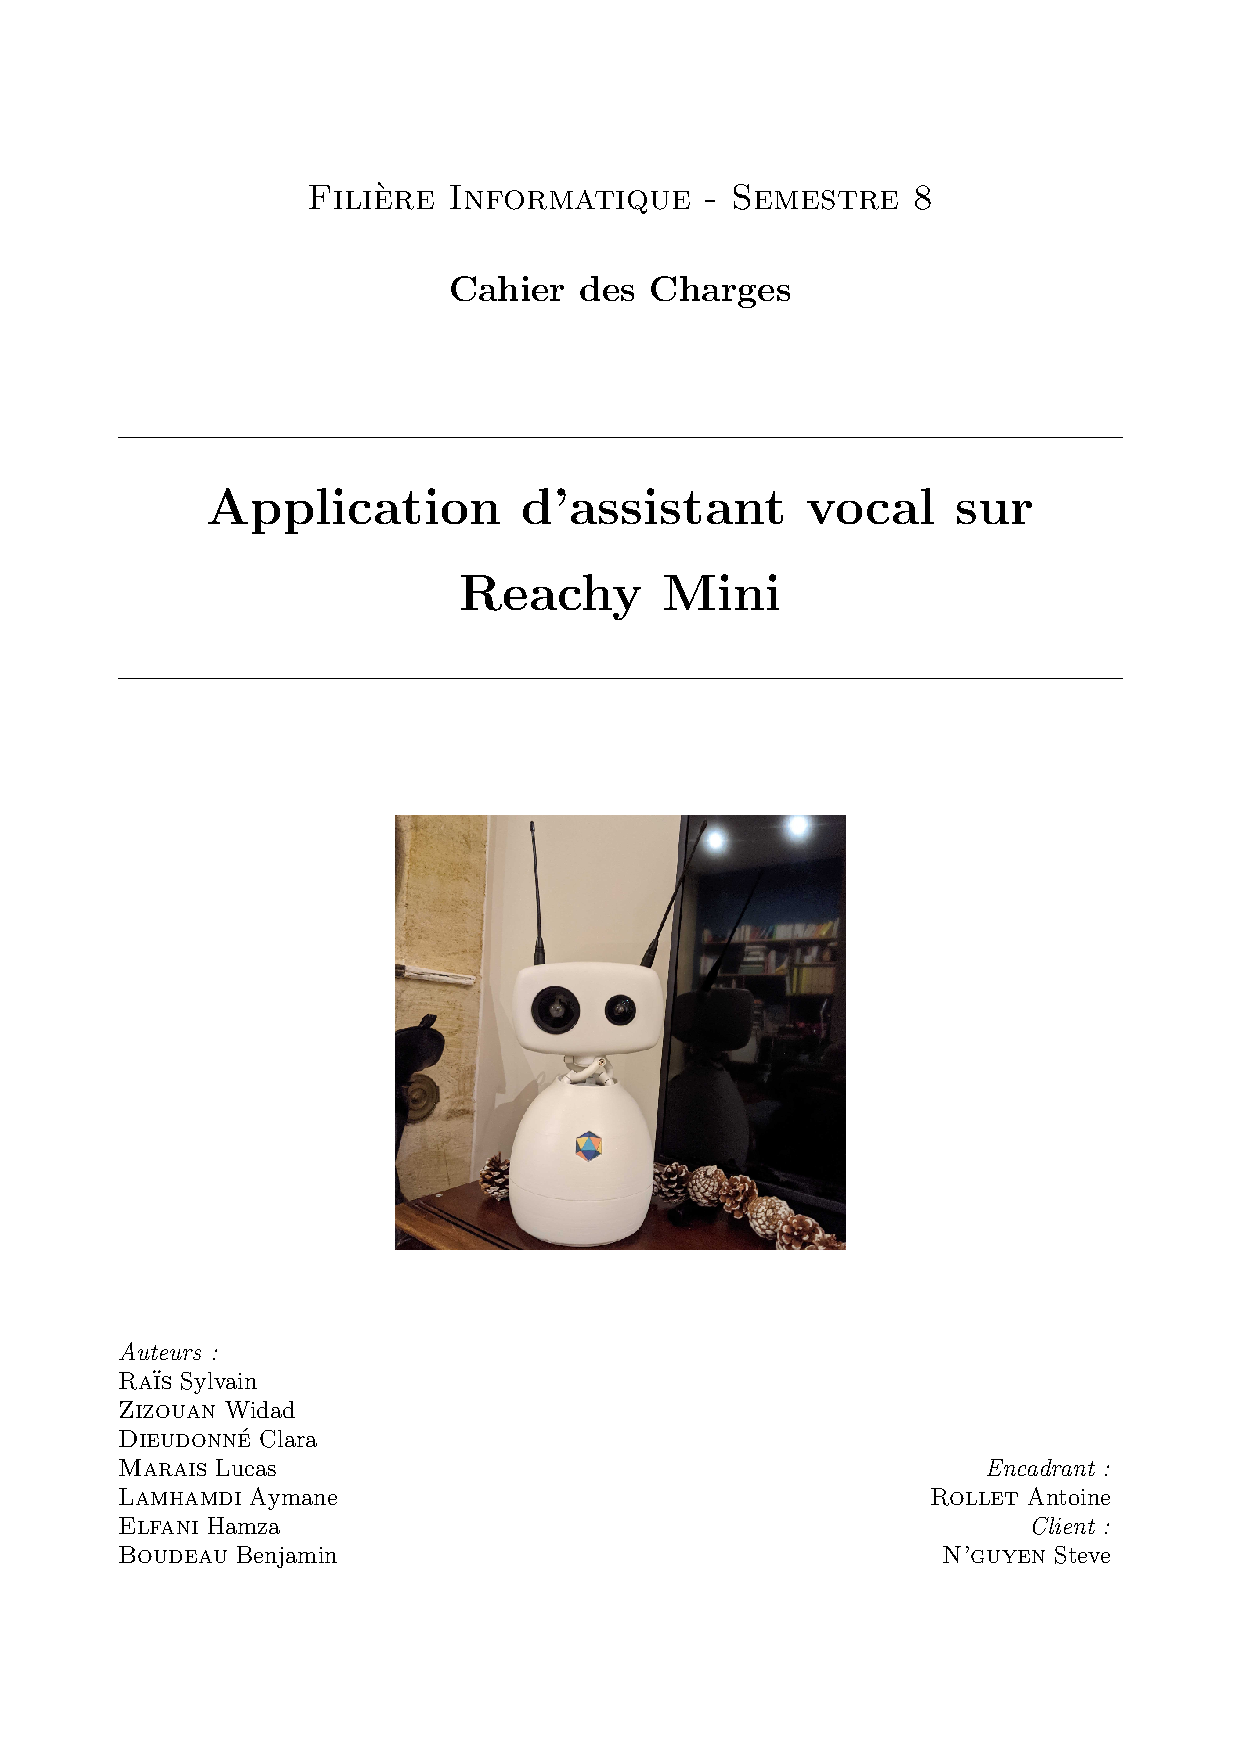
\includepdf[pages=-]{Cahier_des_charges_PFA.pdf}

\subsection{Fichier .json} \label{subsec:annexe_json}

\begin{lstlisting}[language=json,firstnumber=1,caption={Machine à états factice afin de comprendre la structure des \texttt{.json}},captionpos=b]
    {
    "states": {
        "allumage_robot": {
            "action": "allumage_robot_func",
            "transitions": [
                {   
                    "target": "recherche_interaction_only_aruco"
                }
            ]
        },
        "recherche_interaction_only_aruco": {
            "action": "recherche_interaction__only_aruco_func",
            "transitions": [
                {
                    "target": "attente_ordre_only_aruco",
                    "predicat": "activation_aruco_det",
                    "action": "reset_activation"
                }
            ],
            "timeout":{
                "time":120,
                "target":"incitation_aruco"
            }
        },
        "incitation_aruco":{
            "action": "incitation_aruco_func",
            "transitions": [
                {
                    "target": "recherche_interaction_only_aruco"
                }
            ] 
        },
        "eteindre":{
            "action": "eteindre_func"
        },
        "attente_ordre_only_aruco": {
            "action": "attente_ordre_only_aruco_func",
            "transitions": [
                {
                    "target": "traitement_ordre_only_aruco",
                    "predicat": "aruco_verif"
                }
            ],
            "timeout":{
                "time":30,
                "target":"recherche_interaction_only_aruco"
            }
        },
    },
    "module":"reachy_state_machine_100_ans_func"
}

\end{lstlisting}

\end{document}
